\chapter{Modulo Base - Scientifc Python}
\section{\textit{Lun 20 sett - Lezione 1}}
\section{Lecture basic 1: Development workflow}

\subsection{L'importanza della riproducibilità}
La ricerca scientifica dovrebbe essere prima di tutto \textit{corretta} e \textit{riproducibile}. In particolare, \textit{riproducibile} vuol dire che deve essere possibile, partendo dagli stessi dati, arrivare alle stesse conclusioni.\\
Il software ricopre un ruolo fondamentale nella moderna fisica sperimentale. Per questo motivo deve essere trattato alla stregua di un esperimento scientifico, cioè deve essere sviluppato in maniera controllata e deve essere riproducibile.




\subsection{Version control}

“Version control”: \textit{A component of software configuration
management, version control, also known as revision control or
source control, is the management of changes to documents,
computer programs, large web sites, and other collections of
information}\footnote{Wikipedia}\\

Un sistema di Version Control permette di raccogliere metadati\footnote{In informatica il metadato è un sistema strutturato di dati sui dati. Il suo scopo è di descrivere il contenuto, la struttura e l’ambito in cui s’inquadra un documento informatico, per la sua gestione e archiviazione nel tempo.} sul codice ogni qual volta il codice subisce delle modifiche.


\subsection{Terminologia}

  \begin{itemize}
  \renewcommand\labelitemi{--}
  \setlength\itemsep{0.1em}
  \item \textbf{Repository}: the place where files' current and historical data
    are stored
  \item \textbf{Revision or version}: the state at a point in time of the entire
    tree in the repository
  \item \textbf{Clone}: creating a repository containing the revisions from
    another repository
  \item \textbf{Working copy}: a local copy of files from a repository at a
    specific revision
  \item \textbf{Checkout}: create a local working copy from the repository
  \item \textbf{Change or diff}: a specific modification to a set of files under
    version control
  \item \textbf{Commit}: write the changes made in the working copy back to the
    repository
  \end{itemize}


\subsection{Tipologie di Version Control System}
Nel corso degli anni sono state sviluppate diverse tipologie di sistemi di controllo di configurazione. I principali sono i seguenti: \newpage


\subsection{Local version control systems (e.g. RCS)}


\begin{figure}[ht]
    \centering
    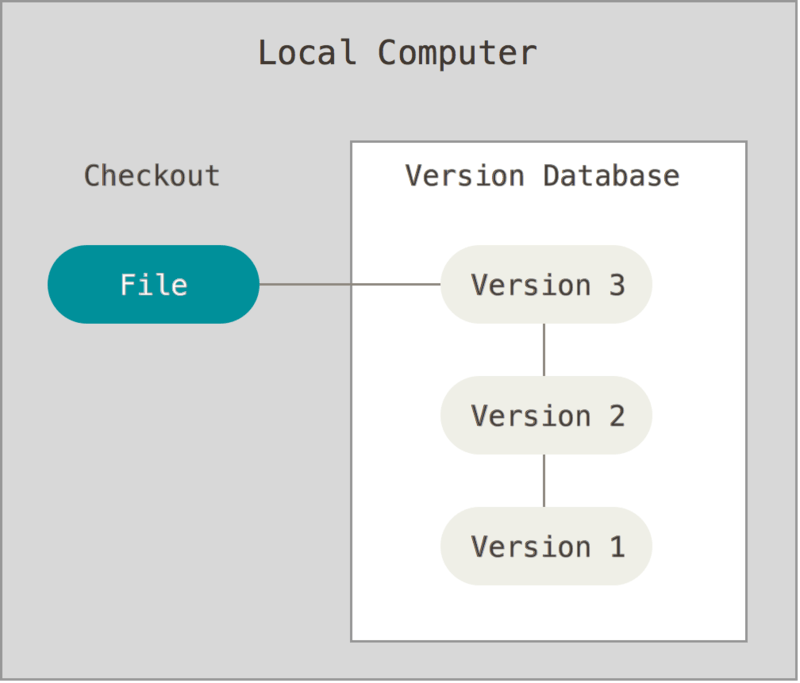
\includegraphics[width=0.5\textwidth]{lez1/localVCS.png}
    \caption{Local version control system: Keeps differences between revisions in a local database. Can recreate what any file looked like at any point in time. }
    \label{localVCS}
\end{figure}
\FloatBarrier


\subsection{Centralized Version Control Systems (e.g. CVS, Subversion)}

\begin{figure}[ht]
    \centering
    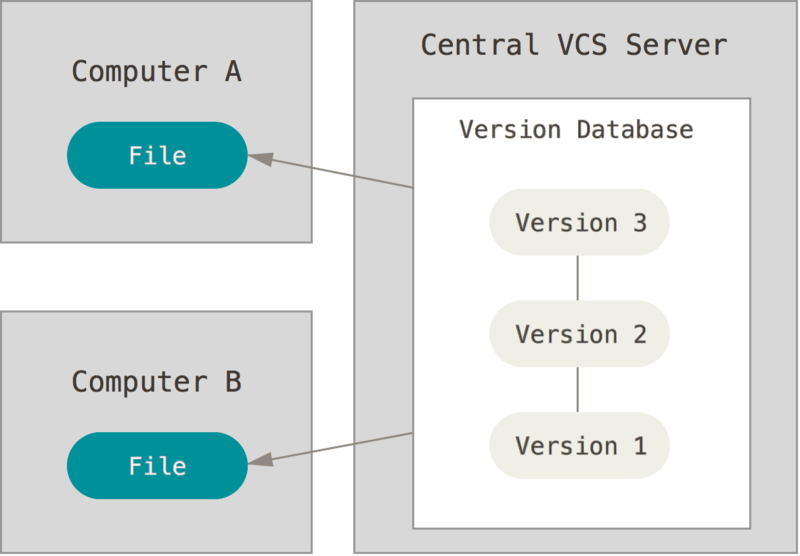
\includegraphics[width=0.5\textwidth]{lez1/centralVCS.png}
    \caption{Centralized Version Control System: Single server containing all the versioned files. Clients can check out the files from the repository. Most popular model through most of the ’90.}
    \label{centralVCS}
\end{figure}
\FloatBarrier

Il work-flow tipico dei Centralized Version Control System è molto basico:
\begin{enumerate}
    \setlength\itemsep{0.1em}
    \item Check out a local working copy from the remote server
    \item Modify the working copy
    \item Commit the changes back to the repository
\end{enumerate}

\newpage
\subsection{Distributed version control system (e.g. git, mercurial)}



\begin{figure}[ht]
    \centering
    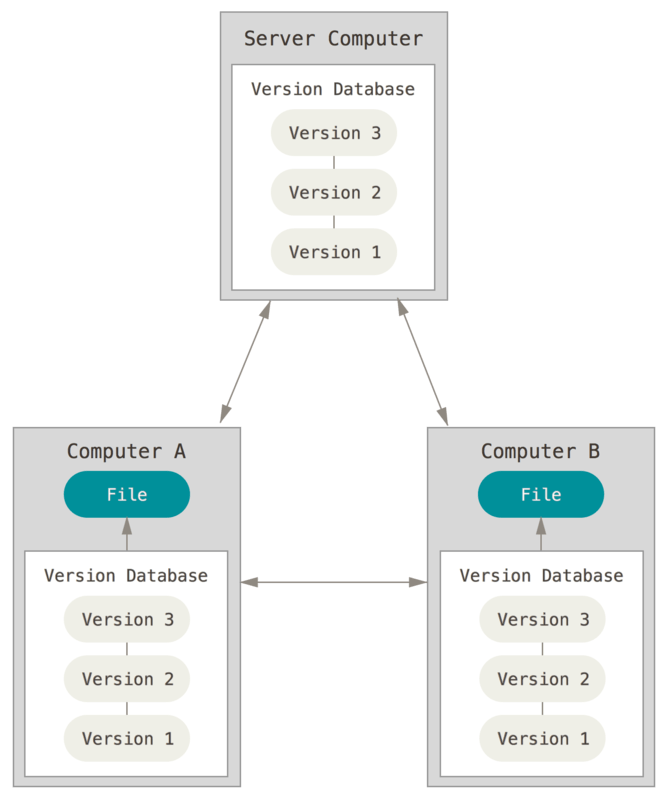
\includegraphics[width=0.5\textwidth]{lez1/distributedVCS.png}
    \caption{Distributed version control system: Clients fully mirror the repository, including its full history. Allows for a much richer variety of work-flows.}
    \label{distrVCS}
\end{figure}
\FloatBarrier


\subsection{Versioning single files vs. the entire repository}

Old VCS only tracked modification on a file-by-file basis; i.e., CVS assigns revision numbers to the single files.
All modern VCS track a whole commit as a new revision; i.e., revisions are assigned to the repository.\\
It makes a lot of sense to version the entire repository.
Versioning single files can give a cozy feeling, but when files interact with each other you need to know the status
of the entire repository to reliably predict the output!



\subsection{Centralized vs. distributed VCS}





\begin{figure}[ht]
    \centering
    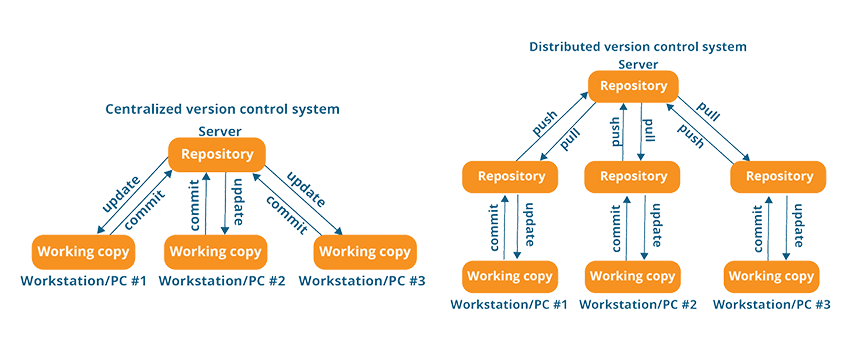
\includegraphics[width=1\textwidth]{lez1/centralvsdistr.png}
    \caption{Confronto tra un sistema di controllo centralizzato ed uno distribuito.}
    \label{confrontoVCS}
\end{figure}
\FloatBarrier

Il workflow nel caso del \textit{centralized VCS} è \textbf{lineare}: \textit{Subversion assigns a progressive number to the repo at each commit.}\\

Invece nel caso di un \textit{Distributed VCS}, il workflow è intrinsecamente \textbf{non lineare}: \textit{Any one given local repository is not ahead or behind any other
repository—just different.}\\
Ma allora come facciamo ad assegnare una versione (revision) in un sistema distribuito? Per capirlo facciamo una piccola digressione sulle funzioni di hash:

\subsection{Funzioni di Hash}

Nel linguaggio matematico e informatico, l'hash è una funzione non invertibile che mappa una stringa di lunghezza arbitraria in una stringa di lunghezza predefinita. Esistono numerosi algoritmi che realizzano funzioni hash con particolari proprietà che dipendono dall'applicazione.\footnote{Wikipedia}

\begin{figure}[ht]
    \centering
    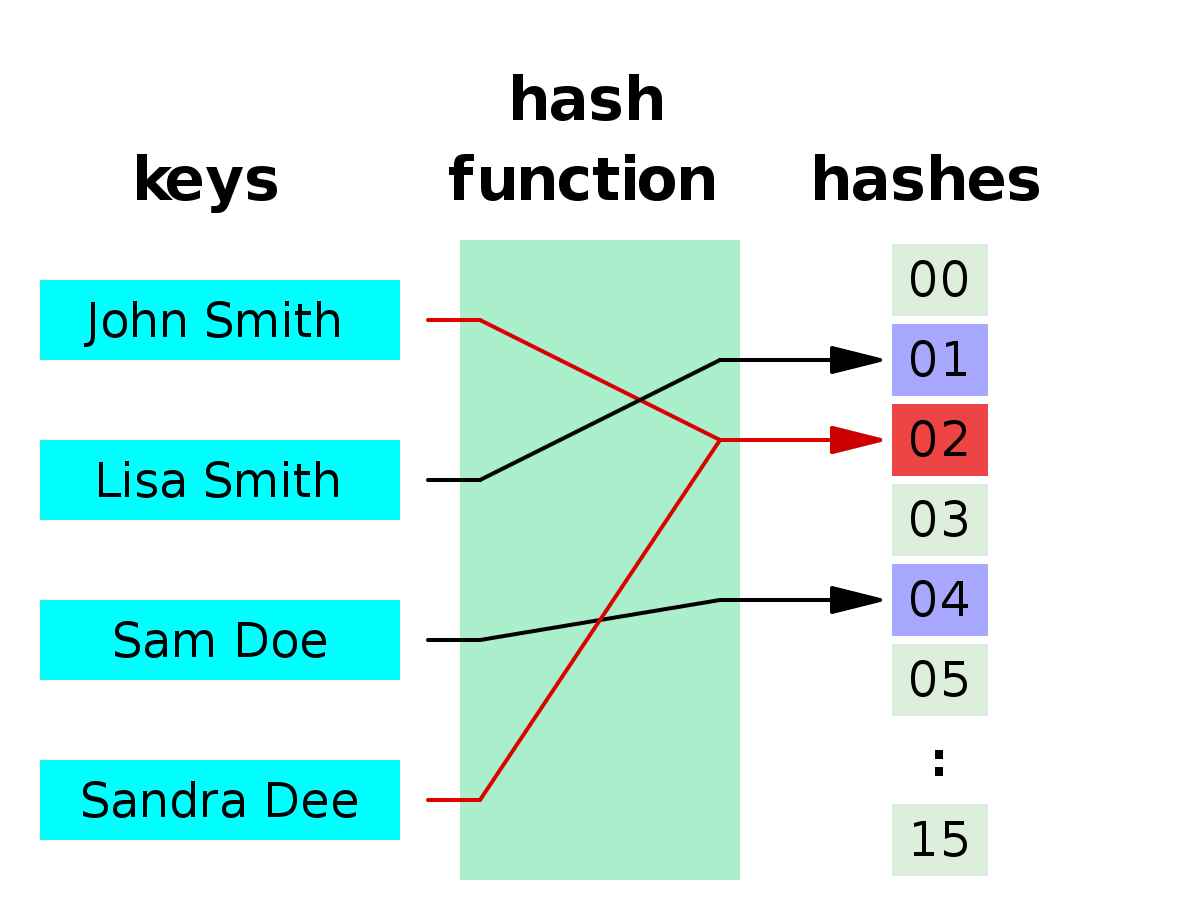
\includegraphics[width=0.5\textwidth]{lez1/hash.png}
    \caption{Esempio di funzione di hash.}
    \label{hash}
\end{figure}
\FloatBarrier


\textit{Hash function maps data of arbitrary size to fixed-size values (e.g., anything to an integer).}\\

Alcune proprietà che deve avere una buona funzione di hash:

\begin{itemize}
\renewcommand\labelitemi{--}
\setlength\itemsep{0.1em}
\item Deterministica.
\item Uniforme nello spazio immagine (minimicca le collisioni).
\item Facile da calcolare (e, possibilmente, difficile da invertire).
\end{itemize}


% \inputminted[frame=lines,framesep=2mm,bgcolor=LightGray]{python}{snippets/hashing.py}

\begin{minted}
[
frame=single,
framesep=2mm,
baselinestretch=1.2,
fontsize=\footnotesize,
linenos
]
{python}
print(hash(3))
print(hash(3.))
print(hash(3.001))
print(hash(’hello’))
print(hash(’Hello’))

[Output]
3
3
2305843009213443
-8080512805622017032
-8706679013462221575
\end{minted}

Every immutable object is hashable in Python. Each type gets its own algorithm.
This is important because in distributed VCS each commit gets its own hash.




\subsection{Altra Terminologia}

\begin{figure}[ht]
    \centering
    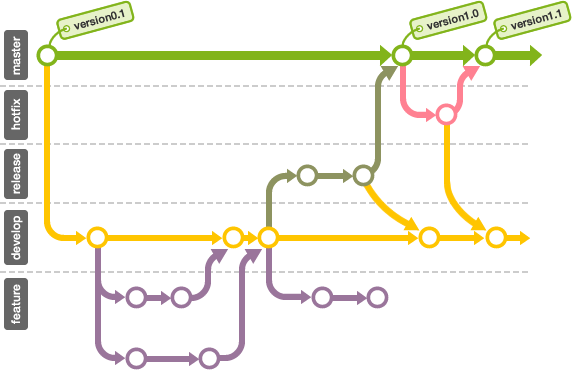
\includegraphics[width=0.5\textwidth]{lez1/branching.png}
    \caption{Esempio di branching.}
    \label{branching}
\end{figure}
\FloatBarrier


\begin{itemize}
  \renewcommand\labelitemi{--}
  \setlength\itemsep{0.1em}
  \item \textbf{Branches:} alternative paths where more copies of the same files develop in different ways independently.
  
  \item \textbf{Master, or trunk, or tip:} the unique line of development that is not a branch.
  
  \item \textbf{Merge:} application of two sets of changes to a set of files.
  \item \textbf{Conflict:} changes to the same file by two or more developers that
the system is unable to reconcile.
  \end{itemize}

\newpage
\section{\textit{Gio 22 sett - Lezione 2}}
\section{Lecture basic 2: Python Basics (1/2)}

\subsection{PEP: Python Enhancement Proposal}

\textit{"PEP stands for Python Enhancement Proposal, and there are several of them. A PEP is a document that describes new features proposed for Python and documents aspects of Python, like design and style, for the community."}

\subsection{Coding Conventions}
Ci sono delle linee guida su come scrivere il codice. Queste si chiamano \textit{Coding Conventions}, e differiscono per ogni linguaggio.\\
In particolare la \textbf{PEP8}\footnote{dargli un'occhiata \url{https://peps.python.org/pep-0008/}} codifica la coding convention in python.\\

Un esempio può essere quello di usare per le indentazioni gli spazi anziché i tab. Questo perché il tab dipende dall'editor di testo usato e questo è un male!\\

Esistono dei tool che permettono di controllare automaticamente quanto un codice è \textit{Pythonico}, ad esempio \textbf{pylint}\footnote{\url{https://www.pylint.org/}}.
\'E buona abitudine, prima di pushare un file su github, usare pylint per controllare che non ci siano errori nel codice!.


\subsection{Variables and basic types}
Python è quello che si chiama \textit{linguaggio tipizzato forte}\footnote{In un linguaggio fortemente tipizzato, il programmatore è tenuto a specificare il tipo di ogni elemento sintattico che durante l'esecuzione denota un valore (per esempio un valore costante, una variabile o un'espressione), e il linguaggio garantisce che tale valore sia utilizzato in modo coerente con il tipo specificato: per esempio, non è possibile eseguire una somma aritmetica su dati di tipo stringa. Questo concetto generale può applicarsi con diverse sfumature; a seconda del contesto.}.
Nonostante ciò, in python le variabili non si dichiarano. Posso scrivere:

\begin{minted}
[
frame=single,
framesep=2mm,
baselinestretch=1.2,
fontsize=\footnotesize,
linenos
]
{python}
x = 3
x = 'ciao'
\end{minted}

senza che mi dia errore.\\
Invece in C (così come nella maggior parte dei linguaggi compilati), una volta dichiarata una variabile, essa è di quel tipo per sempre!\\

Vediamo ora le principali strutture dati di python. Ricordiamo che le strutture dati si differenziano in mutabili e immutabili. In particolare, le strutture dati sono definite dalle operazioni che ci posso fare sopra.\\

\begin{itemize}
    \item \textbf{Numeri} (Interi, Float): notiamo che in python esiste un solo tipo di interi, detto "a precisione illimitata": posso rappesentare un numero arbitrariamente grande finché non finisco la RAM.\\
    \item \textbf{Stringhe}: è equivalente usare le virgolette singole (' ') o doppie (" ").
    
    \item \textbf{Liste}: le liste sono sequenze di elementi, che possono essere di qualsiasi tipo, anche liste stesse. Ad esempio posso accedere al primo elemento della lista \texttt{l} facendo \texttt{l[0]}; oppure cambiare un elemento facendo \texttt{l[0]='ciao'}. Infine posso appendere un elemento alla fine facendo \texttt{l.append('last')}.
    
    \item \textbf{Tuple}: ad esempio \texttt{t = (1,2,3)}. Una tupla è come una lista, ma è immutabile. Posso sempre accedere al primo elemento della tupla \texttt{t} facendo \texttt{t[0]}, ma \textbf{non} posso cambiare un elemento facendo ad esempio \texttt{l[0]=33}.\\
    Se scrivo su terminale: \texttt{(1,2,3)+(5,6,7)}, otterrò la nuova tupla \texttt{(1,2,3,5,6,7)}.
    \item \textbf{Dizionari}: Sono oggetti di tipo chiave-valore, ovvero mappano (mediante hash table o albero binario) una chiave in un valore. Sono efficienti nel trovare il valore associato alla chiave. Ad esempio \texttt{'a':3, 'b':4}.
\end{itemize}

Di seguito alcuni esempi:
\begin{minted}
[
frame=single,
framesep=2mm,
baselinestretch=1.2,
fontsize=\footnotesize,
linenos
]
{python}
i = 3
x = 3.0
print(i, type(i))
print(x, type(x))
s = ’Hi there!’
print(s, type(s))
l = [1, 2, ’a string’]
print(l, type(l), l[0])
t = (1, 2, ’a string’)
print(t, type(t), t[0])
d = {’key1’: 1, ’key2’: 2}
print(d, type(d), d[’key1’])
[Output]
3 <class ’int’>
3.0 <class ’float’>
Hi there! <class ’str’>
[1, 2, ’a string’] <class ’list’> 1
(1, 2, ’a string’) <class ’tuple’> 1
’key1’: 1, ’key2’: 2 <class ’dict’> 1
\end{minted}


\subsection{String Formatting}
\'E poco pithonico usare l'operatore \texttt{+} per unire due stringhe, facendo ad esempio \texttt{'Luca' + 'Baldini'}.\\
\'E anche preferibile evitare usare l'operatore \%.\\
La cosa migliore è usare le \textit{f-string}, come si vede nel seguente esempio:


\begin{minted}
[
frame=single,
framesep=2mm,
baselinestretch=1.2,
fontsize=\footnotesize,
linenos
]
{python}

name = 'Luca'
age = 42

# The ugly way.
print('My name is ' + name + ' I am ' + str(age) + ' year(s) old.')

# The old way (% operator)
print('My name is %s I am %d year(s) old.' % (name, age))

# The new way (.format)
# This is actually *much* more powerful and flexible than implied here.
print('My name is {} I am {} year(s) old.'.format(name, age))

# The newer way---new in Python 3.6. This is awesome!
print(f'My name is {name} I am {age} year(s) old.')


[Output]
My name is Luca I am 42 year(s) old.
My name is Luca I am 42 year(s) old.
My name is Luca I am 42 year(s) old.
My name is Luca I am 42 year(s) old.
\end{minted}

\subsection{Le Funzioni}

DRY (Don’t Repeat Yourself) is better than WET (Write Every Time). \'E importante dare un nome chiaro ed esplicativo alle funzioni che scriviamo.


\begin{minted}
[
frame=single,
framesep=2mm,
baselinestretch=1.2,
fontsize=\footnotesize,
linenos
]
{python}
import math
def square(x):
"""Return the square of x.
"""
return x * x
def cartesian_to_polar(x=1., y=1.):
"""Convert cartesian to polar coordinates.
"""
r = math.sqrt(x**2. + y**2.)
phi = math.atan2(y, x)
return r, phi
print(square(2.))
print(cartesian_to_polar(0., 1.))
print(cartesian_to_polar())
[Output]
4.0
(1.0, 1.5707963267948966)
(1.4142135623730951, 0.7853981633974483)
\end{minted}

\subsection{Funzioni Variadiche}
Sono delle funzioni che accettano un numero variabile di argomenti. Ad esempio:

\begin{minted}
[
frame=single,
framesep=2mm,
baselinestretch=1.2,
fontsize=\footnotesize,
linenos
]
{python}
import os
p1 = os.path.join(’path’, ’to’, ’my’, ’file’)
p2 = os.path.join(’howdy’, ’partner’)
print(p1)
print(p2)
s1 = sum([1, 2])
s2 = sum([1, 2, 3, 4, 5])
print(s1)
print(s2)
[Output]
path/to/my/file
howdy/partner
3
15
\end{minted}

\subsection{Arbitrary argument lists}

\begin{minted}
[
frame=single,
framesep=2mm,
baselinestretch=1.2,
fontsize=\footnotesize,
linenos
]
{python}
import os
def join1(*args):
"""Horrible: do not use the + operator with strings in a loop.
"""
out = ’’
for arg in args:
out += ’%s/’ % arg
return out.rstrip(’/’)
def join2(*args):
"""This a more sensible version---and you get the idea of the *.
"""
return ’/’.join(args)
def join3(*args, sep=os.path.sep):
"""Even better---this will work on any OS.
"""
return sep.join(args)
print(join1(’path’, ’to’, ’file’))
print(join2(’path’, ’to’, ’file’))
print(join3(’path’, ’to’, ’file’))
[Output]
path/to/file
path/to/file
path/to/file
\end{minted}

\subsection{Un esempio: la funzione di fit}

\begin{minted}
[
frame=single,
framesep=2mm,
baselinestretch=1.2,
fontsize=\footnotesize,
linenos
]
{python}
import numpy as np
import matplotlib.pyplot as plt
from scipy.optimize import curve_fit
x = np.linspace(0., 10., 11)
y = 2.5 + 3.2 * x
def model(x, m, q):
return m * x + q
popt, pcov = curve_fit(model, x, y)
plt.errorbar(x, y, fmt=’o’)
# Overlay the model without unpacking the best-fit parameters.
plt.plot(x, model(x, *popt))
# Compare with
# mhat, qhat = popt
# plt.plot(x, model(x, mhat, qhat))
\end{minted}

\subsection{Keyword arguments}
Keyword arguments (or named arguments) are values that, when passed into a function, are identifiable by specific parameter names. A keyword argument is preceded by a parameter and the assignment operator, = . Keyword arguments can be likened to dictionaries in that they map a value to a keyword.


\begin{minted}
[
frame=single,
framesep=2mm,
baselinestretch=1.2,
fontsize=\footnotesize,
linenos
]
{python}
def func(**kwargs):
"""
"""
print(kwargs.get(’verbose’, False))
func()
func(verbose=True)
func(verbose=False)
func(verbose=True, num_events=3)
func(True)
[Output]
False
True
False
True
Traceback (most recent call last):
File "snippets/func_kwargs.py", line 11, in <module>
func(True)
TypeError: func() takes 0 positional arguments but 1 was given
\end{minted}

\subsection{Basic control flow}

\begin{minted}
[
frame=single,
framesep=2mm,
baselinestretch=1.2,
fontsize=\footnotesize,
linenos
]
{python}
i = 2
# Conditional expressions
if i == 2:
print(’Apple’)
elif i == 3:
print(’Peach’)
else:
print(’Cheese’)
# For loops
for i in [1, 2, 3]:
print(i)
# While loops
while i != 0:
print(i)
i -= 1
[Output]
Apple
1
2
3
3
2
\end{minted}

\subsection{Advanced Iteration}

\begin{minted}
[
frame=single,
framesep=2mm,
baselinestretch=1.2,
fontsize=\footnotesize,
linenos
]
{python}
list1 = [’a’, ’b’, ’c’]
list2 = [10, 11, 12]
# Horrible (and very un-Pythonic, too)!
for i in range(len(list1)):
print(i, list1[i])
# Nice-looking.
for i, item in enumerate(list1):
print(i, item)
# Zipping iterables
for item1, item2 in zip(list1, list2):
print(item1, item2)
# List comprehension
print([x**2 for x in list2])
[Output]
0 a
1 b
2 c
0 a
1 b
2 c
a 10
b 11
c 12
[100, 121, 144]
\end{minted}

\subsection{Nota: I numeri in virgola mobile sono esatti}
Consideriamo il seguente esempio:
\begin{minted}
[
frame=single,
framesep=2mm,
baselinestretch=1.2,
fontsize=\footnotesize,
linenos
]
{python}
[lbaldini@nbbaldini slides]$ python

Python 3.7.4 (default, Jul 9 2019, 16:32:37)
[GCC 9.1.1 20190503 (Red Hat 9.1.1-1)] on linux
Type "help", "copyright", "credits" or "license" for more information.
>>> 0.1 + 0.2 == 0.3
False
>>> 0.2 + 0.2 == 0.4
True
\end{minted}

Cosa sta succedendo? Il fatto è che, essendo inesatti, non ha senso chiedere se due numeri in virgola mobile siano esatti!\\ Quando scriviamo un numero in virgola mobile, per il PC è sempre un numero raionale, in quanto è troncato.

\subsection{Rappresentazione in virgola mobile}
[...]

\subsection{References}

  \begin{itemize}
  \item\url{https://scipy-lectures.org/}
  \item\url{https://docs.quantifiedcode.com/python-anti-patterns/}
  \item\url{https://sebastianraschka.com/Articles/2014_python_2_3_key_diff.html}
  \item\url{https://www.python.org/dev/peps/pep-0020/}
  \item\url{https://www.python.org/dev/peps/pep-0008/}
  \item\url{https://docs.python-guide.org/writing/style/}
  \item\url{https://docs.python.org/3/library/stdtypes.html}
  \item\url{https://docs.python.org/3/tutorial/controlflow.html\#defining-functions}
  \item\url{https://docs.python.org/3/tutorial/floatingpoint.html}
  \item\url{https://floating-point-gui.de/}
  \item\url{https://www.itu.dk/~sestoft/bachelor/IEEE754_article.pdf}
  \end{itemize}

\section{Lecture basic 3: Python Basics (2/2)}

\subsection{La Python Standard Lybrary}

\begin{itemize}
  \item La gerarchia è sostanzialmtnete la seguente:
    \begin{itemize}
    \item The Python core language (all you get at the interpreter startup)
    \item The Python standard library (e.g., \texttt{math})
    \item An enourmous number of third-party packages (e.g., \texttt{numpy})
    \item Eventuali librerie scritte da noi
    \end{itemize}
  \item The standard library is included in every Python distribution
    \begin{itemize}
    \item And it is (slowly) evolving with time
    \end{itemize}
  \item With third-party packages you are on your own
    \begin{itemize}
    \item Although Anaconda solves many of the issues
    \item And if you are using GNU-Linux your package manager is probably
      taking care of everything for you
    \end{itemize}
  \item (Well---and of course there are your own modules, too\ldots)
  \item Anything that is out of the core is loaded in memory via an
    \texttt{import} statement
  \end{itemize}

\subsection{Il sistema di Import}

\begin{minted}
[
frame=single,
framesep=2mm,
baselinestretch=1.2,
fontsize=\footnotesize,
linenos
]
{python}
from math import *
[...]
# Terrible: where the hell is sqrt coming from?
x = sqrt(2.)
from math import sqrt
[...]
# Better: if you haven’t redefined sqrt this is from the math library
x = sqrt(2.)
import math
[...]
# Best: five more characters, but at least is clear where sqrt is coming from
x = math.sqrt(2.)
\end{minted}

  \begin{itemize}
  \item The \texttt{\$PYTHONPATH} environmental variables is your friend
    to control where you want to import modules from
    \begin{itemize}
    \item You will need to tweak it when you start writing your own packages
    \end{itemize}
  \item You will need suitable \texttt{\_\_init\_\_.py} files to navigate
    directories
  \end{itemize}

\textbf{Nota:} non abusare del sistema di import! Di seguito un esempio ok:

\begin{minted}
[
frame=single,
framesep=2mm,
baselinestretch=1.2,
fontsize=\footnotesize,
linenos
]
{python}
# This is ok, and vastly recognized by the community
import numpy as np
from matplotlib import pyplot as plt
x = np.linspace(0., 10., 100)
y = x**2.
plt.plot(x, y)
\end{minted}

Mentre il seguente esempio è una catastrofe!


\begin{minted}
[
frame=single,
framesep=2mm,
baselinestretch=1.2,
fontsize=\footnotesize,
linenos
]
{python}
from math import *
import logging as log
# ... 1000 lines of code in the middle
x = log(2.)
[Output]
Traceback (most recent call last):
File "snippets/import2.py", line 6, in <module>
x = log(2.)
TypeError: ’module’ object is not callable
\end{minted}

\subsection{La Standard Library: \texttt{time}, \texttt{datetime} and \texttt{calendar}}
\begin{itemize}
  \item Collections of facilities related to date and time
    \begin{itemize}
    \item Measure the execution time of your scripts
    \item Convert from time to date and vice-versa
    \end{itemize}
\end{itemize}
"Il tempo è una cosa seria" -Luca Baldini.

\subsection{La Standard Library: \texttt{math}}

\begin{minted}
[
frame=single,
framesep=2mm,
baselinestretch=1.2,
fontsize=\footnotesize,
linenos
]
{python}
Python 3.7.4 (default, Jul 9 2019, 16:32:37)
[GCC 9.1.1 20190503 (Red Hat 9.1.1-1)] on linux
Type "help", "copyright", "credits" or "license" for more information.
>>> import math
>>> dir(math)
[’__doc__’, ’__file__’, ’__loader__’, ’__name__’, ’__package__’, ’__spec__’,
’acos’, ’acosh’, ’asin’, ’asinh’, ’atan’, ’atan2’, ’atanh’, ’ceil’, ’copysign’,
’cos’, ’cosh’, ’degrees’, ’e’, ’erf’, ’erfc’, ’exp’, ’expm1’, ’fabs’,
’factorial’, ’floor’, ’fmod’, ’frexp’, ’fsum’, ’gamma’, ’gcd’, ’hypot’, ’inf’,
’isclose’, ’isfinite’, ’isinf’, ’isnan’, ’ldexp’, ’lgamma’, ’log’, ’log10’,
’log1p’, ’log2’, ’modf’, ’nan’, ’pi’, ’pow’, ’radians’, ’remainder’, ’sin’,
’sinh’, ’sqrt’, ’tan’, ’tanh’, ’tau’, ’trunc’]
>>>
\end{minted}
\textbf{Nota:} lavorando molto con gli array, ci troveremo ad usare principalmente \texttt{numpy} e \texttt{scipy}.

\subsection{La Standard Library: \texttt{random}}

\begin{minted}
[
frame=single,
framesep=2mm,
baselinestretch=1.2,
fontsize=\footnotesize,
linenos
]
{python}
Python 3.7.4 (default, Jul 9 2019, 16:32:37)
[GCC 9.1.1 20190503 (Red Hat 9.1.1-1)] on linux
Type "help", "copyright", "credits" or "license" for more information.
>>> import random
>>> print(dir(random))
[’BPF’, ’LOG4’, ’NV_MAGICCONST’, ’RECIP_BPF’, ’Random’, ’SG_MAGICCONST’,
’SystemRandom’, ’TWOPI’, ’_BuiltinMethodType’, ’_MethodType’, ’_Sequence’,
’_Set’, ’__all__’, ’__builtins__’, ’__cached__’, ’__doc__’, ’__file__’,
’__loader__’, ’__name__’, ’__package__’, ’__spec__’, ’_acos’, ’_bisect’, ’_ceil’,
’_cos’, ’_e’, ’_exp’, ’_inst’, ’_itertools’, ’_log’, ’_os’, ’_pi’, ’_random’,
’_sha512’, ’_sin’, ’_sqrt’, ’_test’, ’_test_generator’, ’_urandom’, ’_warn’,
’betavariate’, ’choice’, ’choices’, ’expovariate’, ’gammavariate’, ’gauss’,
’getrandbits’, ’getstate’, ’lognormvariate’, ’normalvariate’, ’paretovariate’,
’randint’, ’random’, ’randrange’, ’sample’, ’seed’, ’setstate’, ’shuffle’,
’triangular’, ’uniform’, ’vonmisesvariate’, ’weibullvariate’]
>>>
\end{minted}

Anche qui, useremo principalmente \texttt{numpy}.

\subsection{La Standard Library: \texttt{os}, \texttt{os.path}, \texttt{glob} and
    \texttt{shutil}}
Servono ad interagire con il sistema operativo:

\begin{itemize}
  \item Miscellaneous operating system interfaces
    \begin{itemize}
    \item Access filesystem (access, create and copy files and directories)
    \item List directory content
    \item Environmental variables
    \item Absolute and relative paths
    \item Exec OS commands
    \end{itemize}
  \item All of this in a cross-platform fashion!
  \end{itemize}

\subsection{La Standard Library: \texttt{argparse}}
\'E utilissimo per passare informazioni direttamente dalla linea di comando.
\begin{itemize}
  \item Ever found yourself modifying the source code and running your program with different parameters?
    \begin{itemize}
    \item This is a terribly bad practice!
    \item And git will complain about modified files :-)
    \end{itemize}
  \item Keep the argparse documentation under your pillow!
  \end{itemize}
    
    
\subsection{La Standard Library: \texttt{logging}}  
  \begin{itemize}
  \item Ever found yourself inserting debug print() statements in the code
    when needed?
    \begin{itemize}
    \item This is another terrible bad practice!
    \item And git will complain about modified files :-)
    \end{itemize}
  \item Imagine if there was a thing that:
    \begin{itemize}
    \item allowed to label messages with different levels of severity
      (e.g., debug, info, warning, error)
    \item dynamically set a global filter on the severity level
      (e.g., do not print debug messages)
    \end{itemize}
  \item This thing exists and is called \texttt{logging}
  \item Always prefer \texttt{logging} over \texttt{print}
  \end{itemize}

Esiste anche un altro modulo molto usato che si chiama \texttt{Loguru}. Permette anche di stampare i log su un \textbf{logfile}.

\subsection{Typical layout of a Python package} 
Say you have a project called sample:
\begin{minted}
[
frame=single,
framesep=2mm,
baselinestretch=1.2,
fontsize=\footnotesize,
linenos
]
{python}
README.rst
LICENSE
setup.py
requirements.txt
sample/__init__.py
sample/core.py
sample/helpers.py
docs/conf.py
docs/index.rst
tests/test_basic.py
tests/test_advanced.py
\end{minted}
\begin{itemize}
  \item Here is how the repository layout might look like:
    \begin{itemize}
    \item README.rst
    \item LICENSE (when in doubt use GPL v3)
    \item requirements.txt (dependencies, for pip)
    \item sample (actual python code, note it's the same name as the project)
    \item docs (documentation)
    \item tests (unit tests)
    \end{itemize}
  \item We shall talk a lot about installation, documentation and unit tests
    in the second part of the course (advanced Python)
  \end{itemize}

\subsection{References}
\begin{itemize}
  \item \url{https://docs.python.org/3/library/}
  \item \url{https://pypi.org/}
  \item \url{https://docs.python.org/3/reference/import.html}
  \item \url{https://docs.python-guide.org/}
  \item \url{https://docs.quantifiedcode.com/python-anti-patterns/}
  \end{itemize}

\newpage
\section{\textit{Gio 29 sett - Lezione 3}}
\section{Lecture basic 4: Algorithms and data structures}

Un algoritmo è una sequenza di istruzioni che dicono in modo \textbf{non ambiguo} come risolvere un problema.
Usare un algoritmo piuttosto che un altro può comportare una grande differenza in termini di efficienza di tempi.
\begin{itemize}
  \item Algorithms can be expressed in several different ways:
    \begin{itemize}
    \item Flowcarts
    \item Pseudo-code
    \item Working code snippets
    \end{itemize}
  \item The sequence of operation must be expressed \textbf{unambigously}
  \end{itemize}

\subsection{Esempio: ricerca sequenziale vs ricerca binaria}
\textbf{Problema: trovare un elemento in una lista ordinata.}\\
Posso fare 2 cose:\\
\textbf{1. Forza bruta:} Faccio un loop sulla lista finché non trovo (o no) l'elemento cercato. Questo diventa sempre più sconveniente man mano che la lista si allunga (se la lista è lunga N, in media dovrò controllare N/2 elementi).\\

\textbf{2. Ricerca Binaria:}
    \begin{itemize}
    \item Start from the middle (if that's the target you're done)
    \item If the target is smaller (larger) than the element in the center,
      bisect the half-list on the left (right)
    \item Iterate until you've found the target (or exhausted the list)
    \end{itemize}
In questo caso dovrò controllare in media $\log_2(n)$ elementi. \textbf{Il logaritmo fa una bella differenza!}\\


\subsection{Complessità di un algoritmo}
\textbf{Misura del costo computazionale di un algoritmo.} Lo quantifico come funzione della grandezza dell'input che noi diamo all'algoritmo. Per es se il nostro algoritmo agisce su una lista, è interessante vedere come scala il tempo di operazione in funzione della lunghezza della lista.\\
\textbf{Ordine di grandezza del numero di istruzioni elementari} è una buona stima del tempo di esecuzione del programma. (anche se le istruzioni elementari possono durare un po' diversamente da pc a pc e da linguaggio a linguaggio).\\
Il numero di istruzioni fondamentali che un algoritmo esegue dipende dai dati che gli diamo in ingresso (ad es, a parità di lunghezza della lista, dipende da come è ordinata la lista stessa). Posso comunque chiedermi cosa succede nel \textit{best case}, nel \textit{worst case} e in \textit{average}.

\begin{minted}
[
frame=single,
framesep=2mm,
baselinestretch=1.2,
fontsize=\footnotesize,
linenos
]
{python}
def find_maximum(list_):
"""Find the biggest element in a list.
"""
maximum = list_[0]
for value in list_[1:]:
if value > maximum:
maximum = value
return maximum

l = [1, 2, 5, 98, 3, 1672, 6, 34, 651]
print(find_maximum(l))

[Output]
1672
\end{minted}

  \begin{itemize}
  \item Example: find the largest element in a list of length $n$
  \item How many fundamental instructions is this code executing?
    \begin{itemize}
    \item \textcolor{teal}{(You should realize this is an ill-posed question)}
    \item One assignment and one list lookup at the beginning: $2$
    \item One lookup, one assignment and one comparison for each iteration
      in the for loop: $3(n - 1)$
    \item A variable number of assignments: between $0$ and $(n - 1)$
    \item One final return instruction: 1
    \end{itemize}
  \item \textcolor{teal}{Answer: anything between $3n$ and $4n - 1$}
    \begin{itemize}
    \item (Depending on the input list)
    \end{itemize}
  \end{itemize}

\begin{itemize}
  \item Message \#1: \textcolor{teal}{the exact number of fundamental instructions that an
    algorithm performs is not determined a priori}
    \begin{itemize}
    \item It depends on the input data, instead
    \item And so does the running time
    \end{itemize}
  \item There's a few questions that you can legitimetely ask, anyway
    \begin{itemize}
    \item How many instructions in the \textcolor{teal}{worst case}?
    \item How many instructions in the \textcolor{teal}{best case}?
    \item How many instructions on \textcolor{teal}{average}?
    \end{itemize}
  \item Message \#2: \textcolor{teal}{the \emph{exact} number of operations doesn't really
    matter}, does it?
    \begin{itemize}
    \item Different machines have different executions speed
    \item Different languages have different meaning of
      \emph{fundamental instruction}
    \end{itemize}
  \item Message \#3: still, \textcolor{teal}{the running time is related to the number
  of fundamental instructions}
  \end{itemize}

\subsection{Andamento asintotico e notazioni O-grandi}

\begin{itemize}
  \item Say you have an algorithm operating on an input of lenght $n$
    \begin{itemize}
    \item e.g., a list with $n$ elements
    \item or a string with $n$ characters 
    \end{itemize}
  \item How many fundamental instructions $N$ does it take to for your algorithm
    to run?
    $$
    N = f(n)
    $$
  \item \textcolor{teal}{Asymptotic behavior}: drop all the terms that grow slowly with
    $n$ and only keep the one that grows faster
    $$
    4n - 1 \approx 4n \quad\text{and}\quad 2n^2 + 6n + 3 \approx 2n^2
    $$
    (for large $n$)
  \item Let's go one step further, and say that we neglect the multiplicative
    factor in front of the leading term (posso ignorare il fattore moltiplicativo perché tanto non c'è una corrispondenza 1 ad 1 tra il numero di op elementari e il tempo).
    $$
    4n - 1 \approx n \quad\text{and}\quad 2n^2 + 6n + 3 \approx n^2
    $$
  \item \textcolor{teal}{big-O notation}: the two algorithms are $O(n)$ and $O(n^2)$
  \end{itemize}



\textbf{NB:} Se un algoritmo ha complessità $n^2$
se ho un input 10 volte più grande, il tempo impiegato sarà 100 volte più grande. (\textbf{un algoritmo di complessità $n^2$ fa schifo})


\begin{figure}[ht]
    \centering
    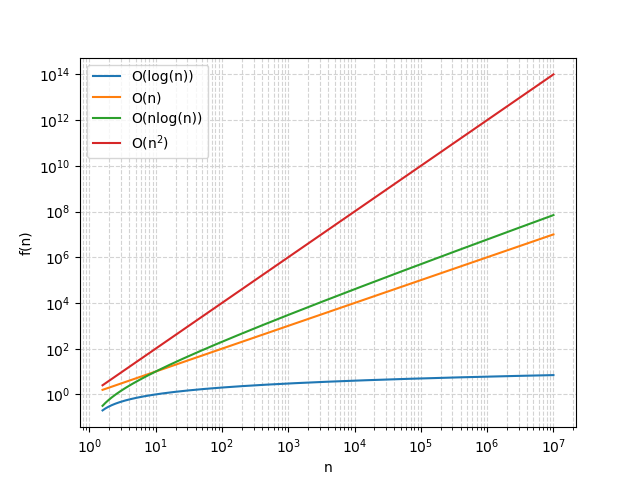
\includegraphics[width=0.8\textwidth]{lez3/asymptotic_behavior.png}
    \caption{Andamenti asintotici di vario tipo. If $n = 10^6$ and you can beat down the complexity from $n^2$ to $n\log(n)$ you are cutting down the execution time by one million!}
    \label{asympt}
\end{figure}
\FloatBarrier

\subsection{Come misuro il comportamento asintotico?}
Soprattutto in casi in cui ci sono un sacco di linee di codice.
\begin{itemize}
    \item \textbf{Forza Bruta}
        \begin{itemize}
        \item Implement the algorithm
        \item Run it on input data of different size and time the run
        \item (Be careful: results may vary from run to run)
        \item Plot the running time vs. input size
    \end{itemize}
    \item \textbf{Per Analisi}:
        \begin{itemize}
        \item Go ahead and count the instructions
        \item Evaluate the best, worst and average case
        \item (This can be difficult for complex programs, and subject to the
      hidiosyncrasis of the language)
    \end{itemize}

    \item \textbf{Ad Occhio}
        \begin{itemize}
        \item un loop ha tipicamente un costo O(n)
        \item anche due loop consecutivi hanno costo O(n)
        \item due loop annidati hanno un costo O($n^2$) appena vedo due loop annidati è un cattivo segno! A volte non si possono evitare, a volte sì!
        \end{itemize}
\end{itemize}


Una lettura leggera sulla "Complexity of Songs": \url{http://www.cs.bme.hu/~friedl/alg/knuth_song_complexity.pdf}

\subsection{Strutture dati: le liste}

\begin{figure}[ht]
    \centering
    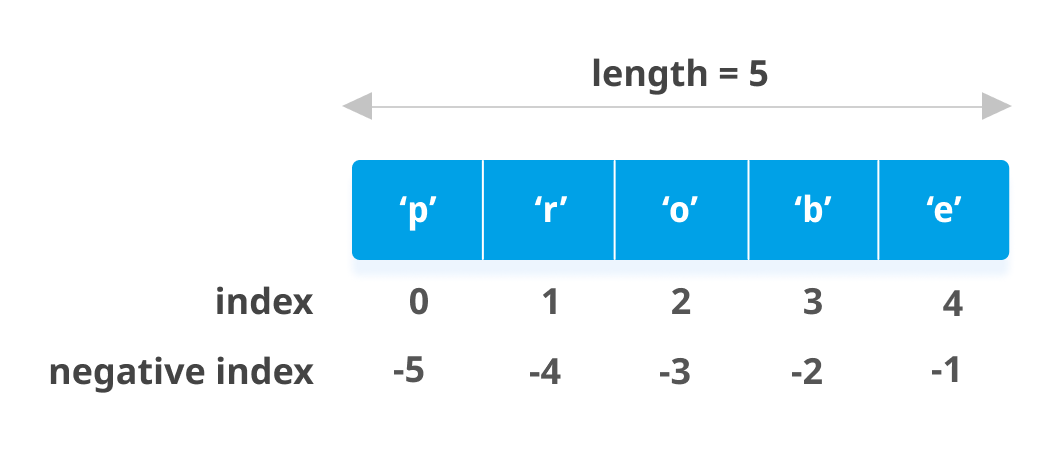
\includegraphics[width=0.7\textwidth]{lez3/list.png}
    \caption{ }
    \label{list}
\end{figure}
\FloatBarrier

\begin{center}

\begin{tabular}{lll}
    \hline
    Operation & Average case & Worst case\\
    \hline
    \hline
    Copy & O(n) & O(n)\\
    Append & O(1) & O(1)\\
    Insert & O(n) & O(n)\\
    Get Item & O(1) & O(1)\\
    Set Item & O(1) & O(1)\\
    Delete Item & O(n) & O(n)\\
    Iteration & O(n) & O(n)\\
    min(s), max(s) & O(n) & \\
    Get Length & O(1) & O(1)\\
    \hline
  \end{tabular}
\end{center}

Quando tolgo un elemento, una volta tolto devo poi rispostare tutto il resto! Per questo ho O(n).
\subsection{Hash table}



\begin{figure}[ht]
    \centering
    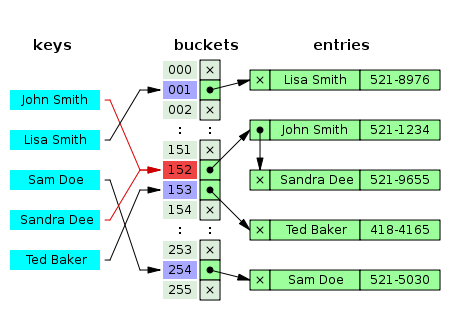
\includegraphics[width=0.7\textwidth]{lez3/hash.png}
    \caption{Hash table}
    \label{hash_table}
\end{figure}
\FloatBarrier

\begin{itemize}
  \item Associative array mapping keys to values
  \item Basic idea:
    \begin{itemize}
    \item Pre-allocate some space (which might grow or shrink)
    \item Keys are mapped to indices via a hash function
    \item This is about it, except that you have to be able to handle collisions
    \end{itemize}
  \item Hash tables (aka dictionaries) are highly optimized in Python
  \end{itemize}

\subsection{Strutture dati: I dizionari}


\begin{figure}[ht]
    \centering
    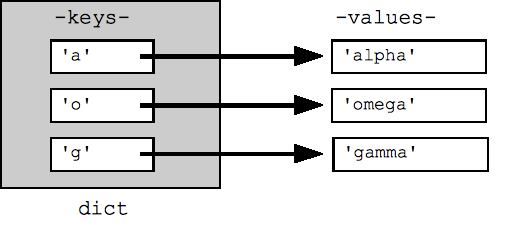
\includegraphics[width=0.6\textwidth]{lez3/dict.png}
    \caption{Dizionario}
    \label{dict}
\end{figure}
\FloatBarrier

\begin{center}

\begin{tabular}{lll}
    \hline
    Operation & Average case & Worst case\\
    \hline
    \hline
    Copy & O(n) & O(n)\\
    Get Item & O(1) & O(n)\\
    Set Item & O(1) & O(n)\\
    Delete Item & O(1) & O(n)\\
    Iteration & O(n) & O(n)\\
    \hline
  \end{tabular}
    
\end{center}

Per prendere un elemento, se non ci sono conflitti mi basta calcolare la funzine di hash sulla chiave. Ma se ci sono dei conflitti, nel caso peggiore in cui la struttura è piena, avrò n conflitti O(n).\\
I dizionari brillano nell'inserzione e nella cancellazione. I dizionari sono ottimi per i contesti in cui devo spesso inserire e/o cancellare cose.

\begin{minted}
[
frame=single,
framesep=2mm,
baselinestretch=1.2,
fontsize=\footnotesize,
linenos
]
{python}
print(hash(3))
print(hash(3.))
d = {}
d[3] = ’Hi there!’
print(d)
d[3.] = ’How are you?’
print(d)

[Output]
3
3
3: ’Hi there!’
3: ’How are you?’
\end{minted}


\begin{itemize}
\item When a float corresponds to an integer, its hash is the same as that of the integer
\item The hash is used to map keys into indices
\item Therefore: $3$ and $3.$ are the same key to a dictionary
\end{itemize}

\subsection{Sorting}
Programma che data una lista di numeri in virgola mobile, mi restituisce un'altra lista con gli stessi elementi, ma in ordine.\\

\begin{minted}
[
frame=single,
framesep=2mm,
baselinestretch=1.2,
fontsize=\footnotesize,
linenos
]
{python}
def sloppy_sort(list_):
"""Poor man’s implementation of a sorting algorithm.
"""
sorted_list = []
for item in list_:
if len(sorted_list) == 0:
sorted_list.append(item)
else:
if item < sorted_list[0]:
sorted_list.insert(0, item)
else:
for i, sorted_item in enumerate(sorted_list):
if item <= sorted_item:
sorted_list.insert(i, item)
break
return sorted_list
l = [10, 1, 5, 2, 7, 3, 9, 4]
print(l)
print(sloppy_sort(l))
[Output]
[10, 1, 5, 2, 7, 3, 9, 4]
[1, 2, 3, 4, 5, 7, 9, 10]
\end{minted}
Questo è un esempio molto brutto per un sort. Infatti contiene 2 for annidati, che corrispondono ad una complessità di ordine $O(n^2)$ (che fa schifo).\\

Esistono diversi algoritmi di sort, di seguito alcuni esempi:
\begin{figure}[ht]
    \centering
    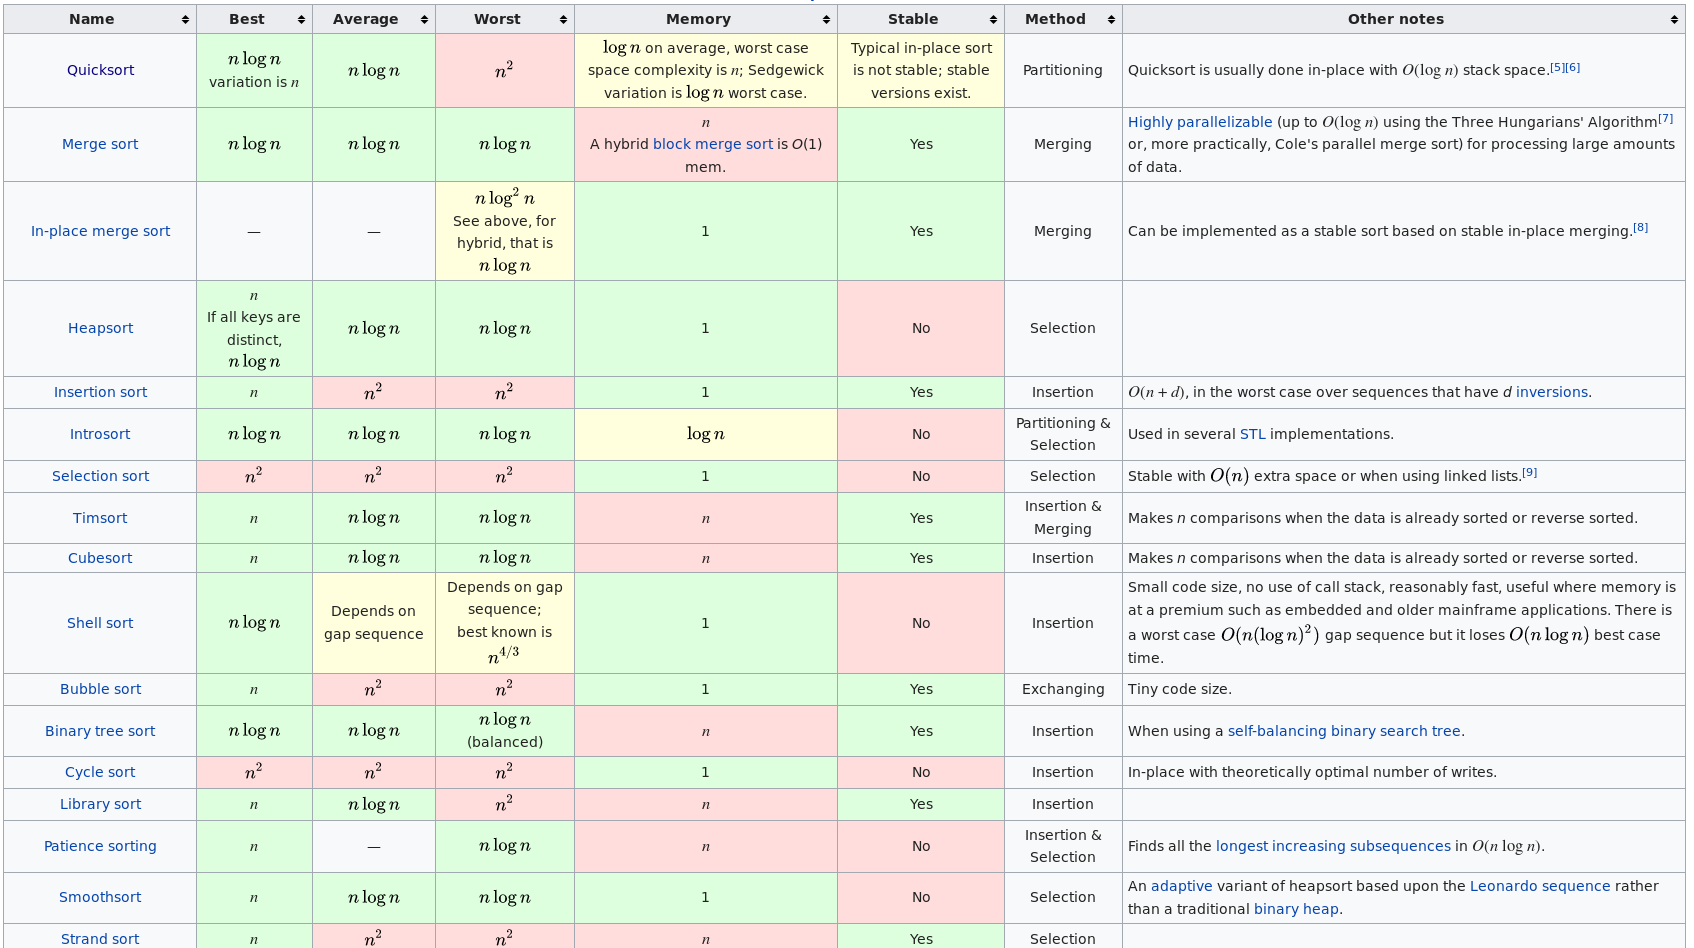
\includegraphics[width=1\textwidth]{lez3/sort.png}
    \caption{Alcuni algoritmi di sort, tabella presa dalla pagina di Wikipedia \url{https://en.wikipedia.org/wiki/Sorting_algorithm}}
    \label{sort}
\end{figure}
\FloatBarrier


Python come algoritmo di sort usa \textbf{Timsort}:
% (comando \texttt{sorted(list)})

\begin{minted}
[
frame=single,
framesep=2mm,
baselinestretch=1.2,
fontsize=\footnotesize,
linenos
]
{python}
l = [10, 1, 5, 2, 7, 3, 9, 4]
print(l)
l.sort()
print(l)

[Output]
[10, 1, 5, 2, 7, 3, 9, 4]
[1, 2, 3, 4, 5, 7, 9, 10]
\end{minted}
\begin{itemize}
  \item Hybrid algorithm, derived from merge sort and insertion sort
    \begin{itemize}
    \item Find subsequences of the data that are already ordered
    \item Use that knowledge to sort the remainder more efficiently
    \end{itemize}
  \item ``Although practicality beats purity'' (The Zen of Python)
  \end{itemize}


\subsection{References}
  \begin{itemize}
  \item \url{https://en.wikipedia.org/wiki/Algorithm}
  \item \url{https://discrete.gr/complexity/}
  \item \url{https://wiki.python.org/moin/TimeComplexity}
  \item \url{https://en.wikipedia.org/wiki/Sorting_algorithm}
  \item \url{https://bugs.python.org/file4451/timsort.txt}
  \item \url{https://en.wikipedia.org/wiki/Timsort}
  \end{itemize}

\section{Lecture basic 7: Numpy e Scipy}



  \begin{itemize}
    \item Among (many) other things, numpy offers:
    \begin{itemize}
    \item a powerful n-dimensional array object
    \item mathematical functions that interoperate natively with arrays
    \end{itemize}
  \item And scipy provides:
    \begin{itemize}
    \item integration
    \item optimization (a.k.a. fitting)
    \item interpolation
    \item signal processing
    \end{itemize}
  \end{itemize}

\subsection{Array di numpy}
Numpy fornisce un'implementazione efficiente di array.\\

Che differenza c'è tra una lista di python e gli array di numpy?
La prima differenza fondamentale è che gli array di numpy sono tendenzialmente \textbf{omogenei} (dentro lo stesso array non posso mescolare due tipi).\\

 
%\pythoncode{snippets/numpy_arrays.py}

\begin{minted}{python}
import numpy as np
# Initialization from a list
a1 = np.array([1., 2., 3])
print(a1)
# Zeros, ones, and fixed values
a2 = np.zeros(10)
a3 = np.ones((2, 2))
a4 = np.full(7, 3.)
print(a2)
print(a3)
print(a4)
# Grids
a5 = np.linspace(0., 10., 11)
a6 = np.logspace(0., 1., 11)
print(a5)
print(a6)

[Output]
[1. 2. 3.]
[0. 0. 0. 0. 0. 0. 0. 0. 0. 0.]
[[1. 1.]
 [1. 1.]]
[3. 3. 3. 3. 3. 3. 3.]
[ 0. 1. 2. 3. 4. 5. 6. 7. 8. 9. 10.]
[ 1.        1.25892541 1.58489319 1.99526231 2.51188643 3.16227766
3.98107171 5.01187234 6.30957344 7.94328235 10.      ]
\end{minted}

Altro esempio: \texttt{a = np.linspace(1, 10, 10, dtype=int)}\\
\noindent   
Se so che tipo di dati contiene un array, so già in partenza quanta memoria occupa. Questi array di numpy, una volta stanziati, tipicamente mantengono le stesse dimensioni.
\subsection{numpy arrays vs. Python lists}

\begin{minted}{python}
import numpy as np
# arrays and lists seem similar...
l = [1., 2., 3.]
a = np.array(l)
print(l)
print(a)
# ...but they support basic arithmetic in a different fashion
print(l + l)
print(a + a)

[Output]
[1.0, 2.0, 3.0]
[1. 2. 3.]
[1.0, 2.0, 3.0, 1.0, 2.0, 3.0]
[2. 4. 6.]
\end{minted}

 \begin{itemize}
  \item arrays and lists are fundamentally different objects
    \begin{itemize}
    \item different footprint in memory, operate at different speed
    \item arrays are homogeneous, lists don't need to
    \item arrays offer a much more powerful indexing/slicing
    \item arrays interoperate with numpy mathematical functions
    \end{itemize}
  \end{itemize}
  
\subsection{Broadcasting}
Broadcast vuol dire che su questi array posso fare delle operazioni (ad es somma di due array di stessa lunghezza).\\

\begin{minted}{python}
import numpy as np
a1 = np.array([1., 2.])
a2 = np.array([[1., 2.], [3., 4.]])
c = np.pi
print(a1)
print(a2)
print(c)
print(a1 * a1)
print(a1 * c)
print(a1 * a2)
[Output]
[1. 2.]
[[1. 2.]
[3. 4.]]
3.141592653589793
[1. 4.]
[3.14159265 6.28318531]
[[1. 4.]
[3. 8.]]
\end{minted}
Under certain conditions, numpy can make operations on arrays of different shape. This is extremely useful when vectorizing problems.\\

Con numpy posso fare cose fantasmagoriche del tipo:\\

\begin{minted}{python}
c = np.array([[1,2],[3,4]]\\
c = np.linspace(1,16,16).reshape((4,4))
\end{minted}

\textbf{Nota:} Ogni volta che operiamo su array, l'operazione avviene in C (perché il C è molto più veloce di python).
Sostituire un loop esplicito in python con un operazione tra array di numpy è una cosa ottima in termini di efficienza! Questa cosa si chiama \textbf{vettorizzazione}.\\
Consideriamo il seguente ciclo for:\\

\begin{minted}{python}
for v1, v2 in zip(v1, v2):
s += vi * v2}
\end{minted}


\noindent
dove \texttt{zip( , )} serve per looppare in contemporanea su due cose.\\
Posso fare la stessa operazione usando gli array di numpy:\\

\begin{minted}{python}
s = (v1 * v2).sum()
\end{minted}


\textbf{Ho vettorizzato il problema}. Cioè sono passato da un ciclo for ad un'operazione tra array. Ho ritrovato la velocità del C, mantenendo l'usabilità di python!

\newpage
\section{\textit{Lun 3 ott - Lezione 4}}

\section{Lecture basic: 5 - OOP\footnote{In informatica, la programmazione orientata agli oggetti (in inglese object-oriented programming, in acronimo OOP) è un paradigma di programmazione che permette di definire oggetti software in grado di interagire gli uni con gli altri attraverso lo scambio di messaggi. Particolarmente adatta nei contesti in cui si possono definire delle relazioni di interdipendenza tra i concetti da modellare (contenimento, uso, specializzazione), un ambito che più di altri riesce a sfruttare i vantaggi della programmazione ad oggetti è quello delle interfacce grafiche.} introduction (1/2)}


Una variabile, ad esempio un intero, funge da contenitore per un dato. Ci sono delle strutture dati, come liste e dizionari, che, oltre a contenere dei dati, sono caratterizzate da un set di operazioni che posso fare su di esse.\\

  \begin{itemize}
    \item Working with containers like lists or dictionaries, you may have noticed
          that they can do many thing besides holding the data
    \medskip
    \begin{itemize}
      \item You can extend a list using append() or insert()
      \item Trying to access a non-existent index in a list triggers a specific errror (\emph{IndexError})
      \item You can iterate on a list using the handy for-loop Python syntax
      \item and so on\dots
     \end{itemize}
     \medskip
     \item In other words, a list is a variable that, in addition to its data,
           shows some kind of specific \emph{behaviour}.
     \medskip
     \item How is that implemented?
  \end{itemize}


Si creano delle entità di codice (ogetti) che uniscono ai dati delle funzionalità per operare su di essi. Quindi non solo definiscono come è fatto quel dato in memoria, ma anche come si manipola quel dato.\\
L'idea di base è tenere il codice che opera su i dati e i dati stessi in un unica entià: \textbf{l'oggetto.}\\

Un oggetto è un'entità di codice caratterizzata da:
\begin{itemize}
    \item \textbf{Stato} $\rightarrow$ dati (attributi o membri)
    \item \textbf{Comportamento} $\rightarrow$ implementato tramite funzioni (metodi)
\end{itemize}

La programmazione a oggetti è usatissima, anche se non ovunque. Ad esempio il C non fa uso di programmazione ad oggetti.Comunque, quasi tutti i più importanti linguaggi di programmazione supportano la programmazione ad oggetti.\\

\subsection{Classi e Oggetti}

Una classe è un pezzo di codice che descrive come è fatto un oggetto. Se vogliamo programmare a oggetti dobbimo scrivere delle classi che permettono poi di creare degli oggetti.\\
Una classe è una generalizzazione del concetto di tipo. Ad es. il tipo "intero" si limita a dire quanto spazio occupa in memoria.\\ Quando scriviamo una classe dobbiamo anche descrivere le sue funzionalità (definendo delle funzioni).
Una volta che abbiamo la nostra classe, ad esempio \texttt{"studente"}, possiamo creare uno o più oggetti di tipo \texttt{"studente"}.\\

  \begin{itemize}
  \item Basic defnitions:
    \begin{itemize}
    \item A \alert{class} is a blueprint for creating objects
    \item An \alert{object} is a concrete relization of a class
    \end{itemize}

  \smallskip
  
  \item You can imagine a class like a project, which is used to
        describe how objects are built and how they works

  \smallskip

  \item You can have multiple objects of the same class
  
  \smallskip
  
  \item The relationship is similar to the one between types and variables:
    \begin{itemize} 
    \item A type is an abstract concept, describing how a varibale is
          represented in memory
    \item A variable is a concrete realization of it
    \item You can have several variables of the same type (like several integers
          or several strings)
    \end{itemize}
  
  \smallskip
  
  \item Indeed, to some extent, a class is the generalization of the concept of
        type. It specifies not only how an object \emph{is made} but also how \emph{it behaves}.
  \end{itemize}

\subsection{Esempio: creiamo la classe \texttt{televisione}
}

  \begin{itemize}
  \item Let's consider a familiar object, like a television. It has:
    \smallskip
    \begin{itemize}
    \item A state
      \begin{itemize}
      \item On/off (and possibly standby)
      \item Currently displayed channel
      \item Volume
      \item Brightness, contrast, etc\dots
      \end{itemize}

    \medskip
    
    \item A behaviour
      \smallskip
      \begin{itemize}
      \item Pressing the `power' button will turn ON/OFF
      \item Rotating the volume knob will increase/decrease the volumne
      \item Using the buttons on the remote control will change displayed 
            channel, brightness, contrast etc\dots
      \item And don't forget you need to plug-in before use!
      \end{itemize}
    \end{itemize}
  \end{itemize}

  \begin{itemize}
    \item How would that be represented in the code?
    \smallskip
      \begin{itemize}
      \item The state can be represented by some \alert{attributes} (variables):
      \begin{itemize}
        \item A boolean can represent the ON/OFF state
        \item For the currently displayed channel you can use an integer
        \item Volume, contrast, luminosity etc\dots they all get their own variable(s)
      \end{itemize}

      \medskip
    
      \item The behaviour can be implemented through the \alert{methods}:
      \smallskip
      \begin{itemize}
        \item For example the turn\_on() and turn\_off() functions may change the value of the variable
              and also produce all the related changes (i.e. start/stop video and audio) 
        \item You will probably have the netx\_channel() and previous\_channel() functions for zapping and so on\dots
        \item Of course it can be much more complex than that!
      \end{itemize}
    \end{itemize}
    
    \medskip
    
    \item Attributes and methods are collectively called \alert{members} of the class
    \medskip
    \item Each object of a specific class is an \alert{instance} of that class
  \end{itemize}


%Attributi e metodi si chiamano membri.\\
%Ogni oggetto di una classe specifica è un'\textit{istanza} di quella classe.

\subsection{Python Classes}

Convenzione: le classi le scrivo con l'iniziale maiuscola.\\


\inputminted{python}{snippets/class_tv_basic.py}

\begin{minted}{bash}
[Output]
<class ’__main__.Television’>
True

\end{minted}

In python tutti i tipi sono anche classi. Non esistono tipi di bassissimo livello.\\
Persino le funzioni sono classi.

\inputminted{python}{snippets/everything_is_a_class.py}

\begin{minted}{bash}
[Output]
<class ’int’>
<class ’str’>
<class ’list’>
<class ’function’>
\end{minted}


\subsection{Metodi}
Per definire un metodo, basta definire una funzione dentro una classe.\\
Tutti i metodi di una classe ricevono automaticamente come primo argomento l'oggetto su cui li chiamiamo (\texttt{self}).\\

\inputminted{python}{snippets/class_methods.py}

\begin{minted}{bash}
[Output]
Turning on <__main__.Television object at 0x7fc718217470>
Showing channel 3
\end{minted}

\subsection{Attributi}


\inputminted{python}{snippets/class_attributes_1.py}

\begin{minted}{bash}
[Output]
1
Traceback (most recent call last):
File "snippets/class_attributes_1.py", line 13, in <module>
print(another_tv.x)
AttributeError: ’Television’ object has no attribute ’x’
\end{minted}

\inputminted{python}{snippets/class_attributes_2.py}

\begin{minted}{bash}
[Output]
1
1
\end{minted}

\subsection{Costruttore}

  \begin{itemize}
    \small
    \item Adding attributes like that would be crazy\dots what would happen if I forgot
          to call the 'add\_a\_class\_attribute()' method in the previous example?
    \medskip
    \item Luckily there is a solution for that: the class \alert{constructor}
    \medskip
    \item The constructor is a special method that is called automatically each time
          a class instance is created
    \medskip
    \item A specificity of the constructor is that it cannot return anything
    \medskip
    \item In Python the constructor is the \emph{\_\_init\_\_} method%
          \footnote{Actually the real constructor -- that is the function responsible for 
                    creating the class instances -- is the \emph{\_\_new\_\_} operator, but 99\% of the time you don't need
                    to define that, as all classes have a default one which does the job for you}           
    \medskip
    \item Class methods like \emph{\_\_init\_\_}, with the name surronded by two underscores,
          are called \alert{special} methods or \alert{dunder} methods.
    \medskip
    \item Is is good practice to define all your class attributes inside the constructor!

  \end{itemize}



\inputminted{python}{snippets/class_constructor.py}

\begin{minted}{bash}
[Output]
Creating a television instance...
This is television model Sv32X-553T, owned by Alberto
Creating a television instance...
This is television model Sv32X-553T, owned by Batman
\end{minted}

\subsection{Namespaces}

Python dietro le quinte  è basato su dei dizionari.\\

A \alert{namespace} in Python is a essentially a ditcionary of \emph{unique} names, each one associated to an object (which can be anything: a variable, a function, a class etc\dots).\\
\begin{center}
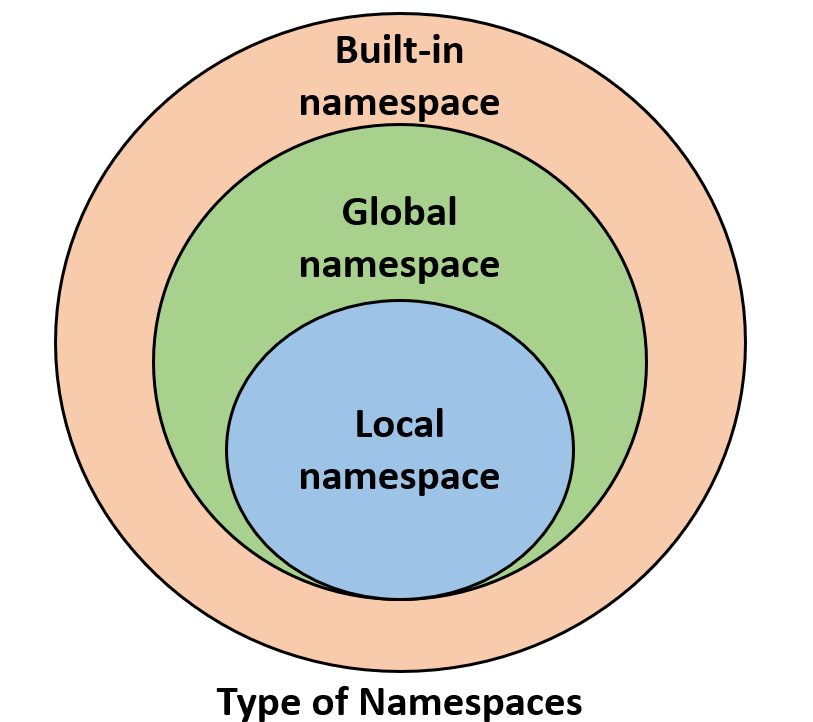
\includegraphics[width=0.25\textwidth]{lez4/namespaces.png}
\end{center}



Python creates separate namespaces for many things: for example, each time a function is called a namespace for local variables is created.\\
You can access objects in the local namespace (and those above -- see picture) just with their name(s); for others you need the '.' (dot) operator.\\

The space of visibility of a variable is called it \alert{scope}.
\subsection{Instance attributes vs class attributes}

  \begin{itemize}
    \small
    \item Each class has a namespace. Plus, each instance of the class get its own additional namespace
    \medskip
    \item The class namespace is automatically visible from each instance namespace, but not the opposite
    \medskip
    \item An attribute in an instance namesespace is an \alert{instance attribute}, and cannot be seen or modified
          by other instances of the class
    \medskip
    \item An attribute in the class namespace is a \alert{class attribute} and is shared among all the instances
    \medskip
    \item Since class attributes are not related to a specific instance, they can be accessed without creating one!
    \medskip
    \item Class attributes are useful to set class constants, or default values, or share data among instances 
  \end{itemize}
  

%Instance attributes: gli elementi della lista hanno ognuno un proprio namespace. 

\subsection{Class attributes (and their strange behaviour)}


\inputminted{python}{snippets/class_attributes_3.py}

\begin{minted}{bash}
[Output]
999
999
998
998
\end{minted}

\hfill
\vfill

\begin{tcolorbox}[width=\textwidth,colback={white},title={Ricapitolando: },colbacktitle=cyan,coltitle=black]
  \begin{itemize}
    \footnotesize
    \item Object Oriented Programming (OOP) is a widespread programming paradigm,
          supported by many programming languages (old and modern), including Python
    \medskip
    \item An object has a state and a behaviour, represented by member variables (attributes)
          and member functions (methods) respectively
    \medskip
    \item A class is a blueprint for creating objects, each object is an instance of a class
    \medskip
    \item In Python classes are defined with the 'class' keyword and instanciated with the '()' operator
    \medskip
    \item Class attributes and methods (globally called members) are accessed through the '.' operator
    \medskip
    \item All the class methods get the object instance as their first argument (usually named 'self')
    \medskip
    \item You should declare class attributes in the constructor a.k.a. the \emph{\_\_init\_\_} function
    \medskip
    \item Instance attributes are not shared: each instance has its own copy of the data
    \medskip
    \item Class attributes are declared outside methods and are shared among all the instances of a class
  \end{itemize} 
\end{tcolorbox}

\newpage


\subsection{Encapsulation - hidden state and interfaces}

C'è un'importante differenza tra interfaccia e implementazione.\\
Pensiamo sempre all'esempio della televisione:




\begin{itemize}
  \item Note that part of the state is hidden from the user (E.g. internal switches, transistors, etc\dots)

  \smallskip
  \item You do not need to know what's going on inside the case to operate a TV!
  \smallskip
  \item All you need to know is how to use the \alert{interface} (the remote
        control, the knobs, the power button, the plug\dots)
  \smallskip
  \item The \alert{implementation} details are hidden: only the TV producer cares about
        them, not the user. 
  \end{itemize}

% Lo stato di un oggetto deve essere modificato   
\begin{itemize}
    \item This leads us to the concept of \alert{encapsulation} 
    \begin{itemize}
      \item \emph{The state of an object should only be accessed and altered
                  through its publicly exposed interface}
    \end{itemize}
    \item That way it is easier to find bugs: you know that, if something is wrong
          with an object, the problem lays inside the class code
    \item That way you can also \emph{enforce behaviour}: for example you can
          prevent from changing the channel if the TV is off
    
\end{itemize}

\textbf{Nota:} una variabile privata è accessibile solo dall'interno della classe.\\

\subsection{Enforcing behaviour}

\inputminted{python}{snippets/class_tv_zapping.py}

\begin{minted}{bash}
[Output]
1
Turning on!
2
\end{minted}

At this point you may be wondering: I can read and modify any class attribute from outside the class using the ’.’ (dot) operator!
Doesn’t that break encapsulation?
Yes it does - but there are ways to fix it!

\subsection{Pythonic encapsulation}


  \begin{itemize}
    \item In languages like C++ you can explicitly declare that some class
          attributes (and methods) are \emph{private}
    \smallskip
    \item In Python there is no concept of \emph{enforced} private attributes
    \smallskip
    \item However, there exists a convention that any attribute/method name prepended by one or two underscore(s) should be considered "private"
    \smallskip
    \item It's like a warning for the class user: you should never access that directly!
    \smallskip
    \item In the case of two underscores Python will actually do a subtle thing to help keeping the data private -- it will 
          prepend \_\emph{classname} to the actual attribute name (see next example)
    \smallskip
    \item However, not everyone in the Python community loves that
    \smallskip
    \item "Never, ever use two leading underscore. This is annoyngly private"\\
           \vspace{0.02\textheight}
           \footnotesize [\emph{Alex Martelli}, member of the Python Software Foundation, author of 'Python in a Nutshell' and co-author of 'The Python cookbook']
  \end{itemize}
  
\subsection{"Private" attributes in Python}

\inputminted{python}{snippets/class_tv_private.py}

\begin{minted}{bash}
[Output]
Sv32X-553T
Alberto
\end{minted}

\subsection{Pythonic encapsulation with properties}

  \begin{itemize}
    \item The possibility of making variables "private" (enforced or not) is not enough of course,
          because sometimes we still want to let the user read or even modify the value of the attribute
    \item The "old" solution for that is providing access functions (the infamous "getters/setters")
    \item But the awsome solution is using \alert{properties} (since Python 2.2)
    \item Properties look similar to getters and setters, but with a twist: you keep
          accessing the attribute with the dot operator
    \item In order to understand why this makes a \emph{huge} difference let's 
          start with an example: suppose you have a class for 2-D vectors
  \end{itemize}

\inputminted{python}{snippets/vector2d_xy.py}

\begin{minted}{bash}
[Output]
3.0 -1.0
3.1622776601683795 -0.3217505543966422
\end{minted}

\begin{itemize}
    \item Suppose you later realize that you use your Vector2d a lot for performing rotations
    \item It would be much faster to store the angle and the module, instead of x and y,
          as the rotation would reduce to a simple addition of the angles
    \item You may think of rewriting your class in that way\dots
  \end{itemize}

\inputminted{python}{snippets/vector2d_rtheta.py}
\noindent In questo caso \texttt{module} e \texttt{angle} sono attributi, mentre \texttt{x} e \texttt{y} sono funzioni.
\begin{minted}{bash}
[Output]
3.1622776601683795 -0.3217505543966422
3.0 -1.0
\end{minted}

  \begin{itemize}
    \item \dots now, however, you have a big problem: your old code is broken!
    \item In every place where your were calling \emph{v.x} or \emph{v.module()}
          now you get an error that needs to be fixed
    \item If other people use your code that is even worse, because you are breaking \emph{their} code
    \item Without properties the solution would have been to design the class from
          the start with private attributes and access functions
  \end{itemize}

\subsection{Old-style encapsulation: never do that!}


\inputminted{python}{snippets/vector2d_old_enc.py}

\begin{minted}{bash}
[Output]
3.0 -1.0
3.1622776601683795 -0.3217505543966422
\end{minted}
  \begin{itemize}
    \item The class data are now "encapsulated", but that is still not ideal:
    \begin{enumerate}
    \item You have written a lot of code just to provide access to a bunch of
          variables
    \item You will have to write even more methods if you want to let the user
          modify that variables as well (e.g. \emph{set\_x(), set\_y()} and so on)
    \item You have to write all this code right from the start, even if you 
          never need it, otherwise you run the risk of getting screwed later
    \end{enumerate}
    \item \alert{properties} solve the problem by \emph{emulating attributes}
  \end{itemize}

\subsection{Properties to emulate attributes}
La property emula l'esistenza di un attributo.

\inputminted{python}{snippets/vector2d_property.py}

\begin{minted}{bash}
[Output]
3.1622776601683795 -0.3217505543966422
3.0 -1.0
\end{minted}

\subsection{Setter properties}

\inputminted{python}{snippets/vector2d_property_setter.py}
Alla riga 25, dietro le quinte sto chiamando il setter (x è un attributo emulato).
\begin{minted}{bash}
[Output]
3.0
1.0000000000000002
\end{minted}

\subsection{Make attributes read-only using properties}


\inputminted{python}{snippets/class_tv_encapsulation_properties.py}

\begin{minted}{bash}
[Output]
This tv belongs to Batman
Nope Joker. Do you want to steal my tv?
This tv belongs to Batman
\end{minted}

\hfill
\vfill

\begin{tcolorbox}[width=\textwidth,colback={white},title={Final note on properties },colbacktitle=cyan,coltitle=black]
  \begin{itemize}
    \item Bottom line: when writing a class, you don't need to make attributes
          private right from the start
    \item You can start with public attributes, and use properties later to
          enforce access/modification rules
    \item That way you only write the code that you really need
  \end{itemize}

Ricapitolando: property permette di fingere che esistano attributi che in realtà non esistono.\\
Inizio con variabili pubbliche. Se in futuro decido di trasformarle in private, definisco una property.\\

Quando scriviamo una classe partiamo con tutte le variabili pubbliche. Dopodiché, se ci accorgiamo ad esempio che una variabile sia di sola lettura: la rendo privata, definisco la property di lettura e poi, volendo, definisco la property di scrittura in modo che mi restituisca un errore.\\
\end{tcolorbox}


\subsection{Interfaccia vs Implementazione}

Quando scriviamo un codice dobbiamo pensarlo in termini dell'interfaccia. \\ L'interfaccia pubblica deve essere più stabile possibile: scrivo il codice in modo da non cambiare l'interfaccia. Nel caso di una classe, gli attributi pubblici fanno parte dell'interfaccia.\\

  \begin{itemize}
    
    \item A physicist thinks:
        
    \medskip
      
    \begin{itemize}
      \item "I have this super-cool algorithm to solve the problem I am working on:
             I will code it carefully, than put together quickly some basic 
             interface to pass data to it and write results to screen / file.
             I need the results quickly for my paper; I can always improve the 
             interface later, right?"
    \end{itemize}
    \medskip
      
    \item A programmer thinks:
    
    \medskip
    
    \begin{itemize}
      \item "I will create a nice interface for the user to handle input/output
             in different formats and I will try to keep it as stable as 
             possible in the future.
             I will start with no algorithm at all -- I will just use random
             numbers to test the interface. I can always implement the
             actual algorithm later, right?"
    \end{itemize}

  \end{itemize}
    
  \begin{itemize}
    \item You don't need to think like a programmer - doing physics is your goal - but
          remember that \alert{interfaces are important}
    \item The concept of interface does not just apply to the program as a whole:
          every significant portion of code (function, class) has its interface
    \item The interface of a class in Python is made by all its "public" members (methods and attributes)
          -- i.e. those without an underscore at the beginning of their name
    \item Changing the interface may break every other piece of code that uses it.
          You want to do that \emph{as less as possible}
    \item You should not access "private" members directly - even if you can. Always
          pass through the interface
    
  \end{itemize}

\hfill
\vfill

\begin{tcolorbox}[width=\textwidth,colback={white},title={Short summary },colbacktitle=cyan,coltitle=black]
  \begin{itemize}
    \small
    \item Encapsulation is the technique of hiding part or all the class state to the user; 
          he can only access and modify that through the class methods
    \medskip
    \item Encapsulation helps debugging by limiting the number of places in the code
          that can mutate the state of an object
    \medskip
    \item It can also be useful to enforce behaviour  
    \medskip
    \item Encapsulation in Python is not enforced by the language, but rather relies on conventions
    \medskip
    \item Class members with an underscore at the beginning of their name are
          considered 'private' and should not be accessed directly oustide the class
    \smallskip
    \item You can use properties to encapsulate your data at any moment in time - never use 'getters' and 'setters'
    \medskip
    \item Interfaces should not change frequently!
  \end{itemize}

\end{tcolorbox}

\newpage

\subsection{Ereditarietà}
L'idea dell'ereditarietà è quella di riutilizzare il più possibile il codice. Funziona creando funzioni specializzate di una classe di partenza.\\
\textbf{Nota:} l'ereditarietà è transitiva.\\

  \begin{itemize}
    \small
    \item Suppose for a moment that you are coding the Monte Carlo for a physics experiment
    \item You want to simulate interactions of charged particles in some detector using OOP paradigm
    \item You may have a class Detetctor and a class for each particle that you need to simulate
    \item Let's say you have a class Electron, a class Positron, a class Proton and a class Alpha
    \item If you think about it, these classes will have a lot of code in common
    \item For example they all need to store their mass, charge, position, velocitiy (or momentum), possibly spin etc\dots
    \item They may also have similar behaviour, though that is less obvious
    \item We know that duplicate code is evil (DRY): how do we avoid that?
  \end{itemize}

  \begin{itemize}
    \small
    \item Many languages - including Python offer a solution for that: \alert{inheritance}
    \item A class can inherit from another one, automatically obtaining all its functionalities (attributes and methods) and then extending or specialyzing them
    \item The class which we inherit from is called \emph{Base} class, \emph{Parent} class or (in Python) \emph{Superclass}
    \item The class inheriting is called \emph{Derived} class or \emph{Child} class
    \item In our problem we can imagine to have a base class 'Particle' and many specialized classes inheriting from it
    \item Inheritance is transtive: if class C inherits from class B, and class B inherits from class A, then class C is also a child of class A (and posses all its functionalities)
  \end{itemize}

\subsection{Inheritance: a basic example}
Nel costruttore della classe figlia si chiama il costruttore della classe madre esplicitamente. Nota: questa chiamata è un po' diversa.\\
\inputminted{python}{snippets/inheritance.py}

\begin{minted}{bash}
[Output]
Energy of e- is 1.1230 MeV/c^2
\end{minted}


\subsection{Overload}
Overload dei metodi: lo stesso metodo lo definiamo sia nella classe madre che nelle classi figlie. Facendo ciò, succede che il metodo nella classe figlia "sovrascrive" il metodo nella classe base.

\inputminted{python}{snippets/overload.py}

\begin{minted}{bash}
[Output]
None
Meow!
Woof!
None
\end{minted}


\subsection{Ereditarietà multipla}

\inputminted{python}{snippets/multiple_inheritance.py}
mro sta per \textit{resolution order}: la classe da cui eredito per prima è la prima in questo ordine di precedenza.

\begin{minted}{bash}
You are listening to channel n. 5
You are looking to channel n. 5
You are listening to channel n. 5
\end{minted}

\textbf{Nota:}Don’t abuse inheritance!\\
In generale: più i pezzi di codice sono indipendenti  e più è facile programmare.

\subsection{Composizione}
Ho come attributo di una classe un oggetto di un'altra classe.\\

  \begin{itemize}
    \item \alert{Composition} is a different technique for reusing functionalities
    \item The concept is simple: just use an object of some class as a member of
          a different one
    \item For example we can create the classes 'Enigne' and 'Wheel' and than 
          the class 'Car' will have a member of type Engine and 4 members of
          type Wheel
    \item A class like 'Car' in the example is sometimes called an 
          \alert{aggregate} class
  \end{itemize}

\inputminted{python}{snippets/composition.py}


\begin{minted}{bash}
[Output]
Broom broom!
\end{minted}


\subsection{Composition vs Inheritance}

la composizione si usa quando voglio rappresentare una classe di appartenenza. Mentre con l'ereditarietà rappresento una relazione diversa: un elettrone eredita dalla classe particella perché un elettrone è una particella.\\
  \begin{itemize}
    \item Composition models a \alert{'has-a'} relation in the real world: a 
          Car \emph{has} a Engine
    \item Inheritance models a \alert{'is-a'} relation in the real world: an
          Electron \emph{is} a Particle
    \item It may not always be obvious which one to use in your specific case:
          choose wisely!
  \end{itemize}
  
Se siamo nel dubbio è meglio usare la composizione: è più safe.


\subsection{Pitfalls of Inheritance}
  \begin{itemize}
    \item Inheritance is a wild beast. There are entire libraries written about how and when (not) to use it
    
    \bigskip
    
    \item Question for you: should a Square inherits from a Rectangle?
    \item Seems legit: a Square \emph{is} a specialized Rectangle
    \item But what happens if the Rectangle class has a changeHeight() method?
    \bigskip
    
    \bigskip
    
    \item \alert{Liskov Substitution Principle}: you should always be able to use
          a derived class instead of a base class in your code
    \item In other words: a derived class should always extend or specialize
          the functionalities of the base class, never restrict them!
   \end{itemize}
   
\hfill
\vfill
  

\begin{tcolorbox}[width=\textwidth,colback={white},title={Short summary },colbacktitle=cyan,coltitle=black]
  \begin{itemize}
    \item A class can inherit funcionalities from one or more other classes (Inheritance)
    \medskip
    \item The class that inherits is call Derived (or Child) class the inherited one is the Base (or Parent) class
    \medskip
    \item Inheritance models an \emph{is-a} relationship
    \medskip
    \item Classes can also incorporate other objects as class members (Composition)
    \medskip
    \item Composition models an \emph{has-a} relationship
    \medskip
    \item Inheritance is tricky: use it with care!
   \end{itemize}

\end{tcolorbox}

\newpage
\section{\textit{Gio 6 ott - Lezione 5}}

\section{Lecture basic: 5 - OOP Introduction (2/2)}

  \begin{itemize}
    \item Suppose we want to create a class for managing 2D vectors\footnote{%
      The content of this lesson is vastly based on the the book '\emph{Fluent Python}' by Luciano Ramalho}
    \item That's just for learning: there are already plenty of libraries for
          doing array operations - like numpy!
    \item Anyway let's start coding some useful methods for it
  \end{itemize}
  

\inputminted{python}{snippets/vector2d_naive.py}
\begin{minted}{bash}
[Output]
Vector2d(3.0, -1.0)
3.1622776601683795
Vector2d(4.0, 0.5)
\end{minted}

  \begin{itemize}
    \item This kind of works but\dots... isn't that ugly?
    \item Look at the lines \emph{v.info()} or \emph{v.module().}
          It would be far more readible to just do \emph{print(v)} and \emph{abs(v)}
    \item And what about \emph{t = v.add(z)}? Why not \emph{t = v + z}?
    \item In Python there is a tool that allows you to do just that: \alert{special methods}
    \item Last lesson we saw that special methods (or dunder methods or 
          magic methods) are methods like \emph{\_\_init\_\_} and got a special
          treatment by the Python interpeter
    \item There are a few tens of special methods in Python. Let's see how they work
  \end{itemize}

\subsection{Special Methods}


\inputminted{python}{snippets/vector2d_2.py}
\begin{minted}{bash}
[Output]
3.1622776601683795
\end{minted}

  \begin{itemize}
    \item And what about \emph{print()}?
    \item There are actually two special methods used for that: \emph{\_\_str\_\_} and \emph{\_\_repr\_\_}
    \item \emph{\_\_str\_\_} is meant to return a concise string for the user; it is called with \emph{str()}
    \item \emph{\_\_repr\_\_} is meant to return a richer output for debug. It is called with \emph{repr()}
    \item \emph{print()} automatically tries to get a string out of the object using \emph{\_\_str\_\_}
    \item If there isn't one, it searches for \emph{\_\_repr\_\_}. A defealut \emph{\_\_repr\_\_}
          is automatically generated for you, if you haven't defined one
  \end{itemize}

\subsection{\emph{\_\_str\_\_} and \emph{\_\_repr\_\_}}

\inputminted{python}{snippets/vector2d_printable.py}
\begin{minted}{bash}
[Output]
(3.0, -1.0)
Vector2d(3.0, -1.0)
I got (3.0, -1.0) with __str__ and Vector2d(3.0, -1.0) with __repr__
\end{minted}

\subsection{Mathematical operations}

\inputminted{python}{snippets/vector2d_math.py}
\begin{minted}{bash}
[Output]
(-2.0, 0.0)
(9.0, -3.0)
(-25.0, 5.0)
\end{minted}

\subsection{In-place operations}
\inputminted{python}{snippets/vector2d_inplace.py}
\begin{minted}{bash}
[Output]
(-2.0, 0.0)
(10.0, 0.0)
\end{minted}

L'addizione fatta con \texttt{\_\_iadd\_\_} è concettualmente diversa da quella fatta con \texttt{\_\_add\_\_}. Infatti in questo caso non sto creando un nuovo vettore, ma sto modificando gli attributi del vettore su cui è chiamata la funzione.

\subsection{Comparisons}

\subsection{In-place operations}
\inputminted{python}{snippets/vector2d_comparable.py}
Alla riga 15 sfruttiamo l'uguaglianza delle \textit{tuple} in modo da risparmiarci l'implementazione from scratch dell'uguaglianza tra float.
\inputminted{python}{snippets/test_vector2d_comparable.py}
\begin{minted}{bash}
[Output]
True False False
False
[Vector2d(3.0, -1.0), Vector2d(-5.0, 1.0), Vector2d(3.0, 0.0)]
[Vector2d(3.0, 0.0), Vector2d(3.0, -1.0), Vector2d(-5.0, 1.0)]
\end{minted}


\subsection{An hashable Vector2d}
  \begin{itemize}
    \item Ok now let's try to make our vector2d \emph{hashable}
    \item Hashable objects can be put in \emph{sets} and used as keys for 
          dictionaries
    \item To make an object hashable we need to fullfill 3 requirements:
    \begin{itemize}
      \item It has to be immutable - otherwise you may not retrieve the correct hash
      \item It needs to implement a \emph{\_\_eq\_\_} function, so one can compare
            objects of this class
      \item It needs a (reasonable) \emph{\_\_hash\_\_} function
    \end{itemize}
    \item Rules for a good hash function:
    \begin{itemize}
      \item Must return the same value for objects that compare as equal
      \item Should rarely return the same value for different objects
      \item Should sample the result space uniformly
    \end{itemize}
    
  \end{itemize}


\inputminted{python}{snippets/vector2d_hashable.py}

\inputminted{python}{snippets/vector2d_hashable_test.py}

\begin{minted}{bash}
[Output]
False True False
-3 -6 -3
Vector2d(-5.0, 1.0), Vector2d(3.0, -1.0)
Vector2d(3.0, -1.0)
\end{minted}

\subsection{Array N-dimensionali}

  \begin{itemize}
    \item 2d array are boring\dots why not a N-d array?
    \item Of course we cannot store the components explicitly like before
    \item We need a container for that and we will use \emph{array} from the 
          array library
    \item This is an example of \alert{composition}
   
    \item Question for you: why not a list or a tuple? $\rightarrow$ Perché le liste sono lente, non sono pensate per fare operazioni matematiche (i dati in memoria non sono contigui) 
    \item Note: \emph{array} uses a typecode (a single character) for picking the
          type. 'd' is the typecode for float numbers in double precision. 
  \end{itemize}
  
  
\inputminted{python}{snippets/vector.py}
A riga 6 stiamo salvando il \texttt{typecode} come attributo della classe: ovvero è condiviso con tutte le istanze della classe.
\begin{minted}{bash}
(5.0, 3.0, -1.0, 8.0)
Vector([5.0, 3.0, -1.0, 8.0])
\end{minted}

  \begin{itemize}
    \item Now that we have an arbitrary number of components, we cannot access them like 
          vector.x, vector.y, \dots anymore
    \item What we want is a syntax similar to that of lists: vector[0], vector[1]
          ans so on
    \item There are two magic methods for that: \emph{\_\_getitem\_\_} for access 
          and \emph{\_\_setitem\_\_} for modifying
    \item While we are at it, we also implement the \emph{\_\_len\_\_} method,
          which allows us to call \emph{len(vector)}
  \end{itemize}
  
\inputminted{python}{snippets/vector_random_access.py}

\inputminted{python}{snippets/test_vector_random_access.py}

\begin{minted}{bash}
[Output]
4
5.0 3.0
Vector([5.0, 10.0, -1.0, 8.0])
Traceback (most recent call last):
    File "snippets/test_vector_random_access.py", line 12, in <module>
        print (v[9]) # This will generate an error!
    File "/data/work/teaching/cmepda/slides/latex/snippets/vector_random_access.py", line 13,
        return self._components[index]
IndexError: array index out of range
\end{minted}  

\subsection{An Iterable Vector}

  \begin{itemize}
    \item Now our vector behaves a bit like a native python list
    \item However a list has a very powerful feature we miss: it's \alert{iterable}
    \item An \emph{iterable} in Python is something that has a
          \emph{\_\_iter\_\_} method, which returns an \alert{iterator}
    \item Technically, an iterator is an object that implements the
          \emph{\_\_next\_\_} special method, which is used to retrieve elements
          one at a time
    \item We will not dicuss iterators any further here: instead, we will just
          exploit composition and borrow the \emph{\_\_iter\_\_} method from the 
          underlying array
  \end{itemize}

\inputminted{python}{snippets/vector_iterable.py}
\begin{minted}{bash}
[Output]
5.1
3.7
-25.0
\end{minted} 

\subsection{Duck Typing\footnote{"If it looks like a duck and quacks like a duck, it must be a duck."}}


\inputminted{python}{snippets/duck_typing.py}

\begin{minted}{bash}
[Output]
Quack!
Quack!
Traceback (most recent call last):
    File "snippets/duck_typing.py", line 20, in <module>
        bird.quack()
AttributeError: ’Penguin’ object has no attribute ’quack’
\end{minted} 


\subsection{Polymorphism}
  
  \begin{itemize}
    \item Reuse the same code for different things
    \item In statically typed languages this is tipically done with inheritance,
          e.g. we make Duck and Goose inherits from a base class QuackingBird()
          or something like that
    \item Python is dynamical, so we can use duck typing for that.
          We just need to implment the quack() method for both Ducks() and Goose() 
          and we are done
    \item In other words we obtain polymorphism just by satsisfying the required \alert{interface}
          (in this case the quack() function)
  \end{itemize}
  
  \subsection{The power of iterables}
  \begin{itemize}
    \item Having an iterable Vector (thanks to the \emph{\_\_iter\_\_} magic
          method) makes all the difference in the world
    \item There are \emph{a lot} of builtin and library functions in python accepting a
          generic iterable as input:
    \begin{itemize}
      \item \emph{sum}: Sum all the elements
      \item \emph{max}/\emph{min}: Return the maximum/minimum
      \item \emph{enumerate}: Iterate with automatic counting of iterations
      \item \emph{map}: Apply a function to the elements one by one
      \item \emph{filter}: Iterate only on the elements passing a given condition
      \item \emph{zip}: Iterate over pairs of elements (requires two iterables)
    \end{itemize}
    \item Countless others can be found in the \alert{\emph{itertools}} library
    \begin{itemize}
      \item \emph{islice}: Slice the loop with start, stop and step
      \item \emph{takewhile}: Stop looping when a condition becomes false
      \item \emph{chain}: Loop through many sequences one after another
      \item \emph{cycle}: Loop over the sequence repeatedly, indefinitely
      \item \emph{permutations}: Get all the permutations of a given length
      \item And so on\dots
    \end{itemize}
    \item With duck typing we can now use any of that for our Vector class -- isn't that cool?
  \end{itemize}

\inputminted{python}{snippets/vector_iterable_test.py}

\begin{minted}{bash}
[Output]
[4.0]
(1.0, 2.0)
(1.0, 4.0)
(2.0, 1.0)
(2.0, 4.0)
(4.0, 1.0)
(4.0, 2.0)
\end{minted} 

\subsection{A vector that behaves like a duck}
\inputminted{python}{snippets/vector_ducked.py}
\inputminted{python}{snippets/test_vector_ducked.py}
\begin{minted}{bash}
[Output]
(1.0, 2.0, 3.0)
3.741657386773941
6.0
False False True
(2.0, 4.0, 8.0)
(2.0, 4.0, 6.0)
\end{minted} 

\subsection{Function are classes}
  
  \begin{itemize}
    \item Remember that in the past lesson I told you that functions are objects
          of the 'function' class.
    \item How are they implemented?
    \medskip
    \item With a special method - of course: \emph{\_\_call\_\_}
    \item Every object implementing a \emph{\_\_call\_\_} method is called \alert{callable}
  \end{itemize}
  
Esempio: Noi tipicamente a \texttt{curve\_fit} passiamo una funzione, ma in realtà possiamo passarle un qualsiasi \textit{callable}!

\subsection{A simple callable for a straight line}

\inputminted{python}{snippets/callable_line.py}
\begin{minted}{bash}
[Output]
y = -2.0 x + 1.0
Slope = -2.0, Intercept = 1.0
-3.0
\end{minted} 

\subsection{Create a call counter}

\inputminted{python}{snippets/callable.py}
Il \textit{"wrapper"} aggiunge un layer di funzionalità intermedie.\\
Riga 16: siccome non conosciamo quali argomenti prende questa funzione, dobbiamo fare in modo che prenda un qualsiasi numero di argomenti.\\

\subsection{Fit hacking}

\inputminted{python}{snippets/test_callable.py}
Riga 15: sto passando a \texttt{curve\_fit} la funzione \textit{"wrappata"}. In questo caso devo per forza passargli p0, altrimenti \texttt{curve\_fit} non ha modo di capire il numero di parametri: tipicamente per capirlo guarda gli argomenti della funzione che gli passiamo, ma in questo caso gli stiamo passando un callable generico!
\begin{minted}{bash}
[Output]
Fitted with 9 function calls
\end{minted} 

\begin{figure}[ht]
    \centering
    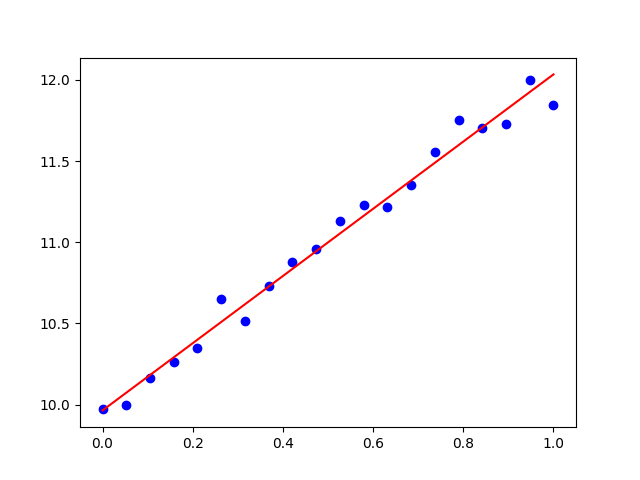
\includegraphics[width=0.6\textwidth]{lez5/fit.png}
    \caption{The fit works as usual}
    \label{fit}
\end{figure}
\FloatBarrier

\vfill
\hfill

\begin{tcolorbox}[width=\textwidth,colback={white},title={Summary: },colbacktitle=cyan,coltitle=black]
  \begin{itemize}
    \item Special methods can beused to greatly enhance the readibility of the code
    \item There are tens of special methods in python, covering logical operations,
          mathematical operations, array-style access, iterations, formatting and
          many other things\dots
    \item Implementing the required interface in your classes you will be able
          to reuse a lot of code written for the standard containers thanks to
          duck typing, which is the pythonic way to polymorphism
   \end{itemize}  
\end{tcolorbox}

\newpage

\section{\textit{Lun 10 ott - Lezione 6}}

\section{Lecture Advanced 1: Testing and documentation}

\subsection{How do I make sure my program is correct?}
In un linguaggio compilato alcune le verifiche le fa il compilatore, che fa per lo meno alcune verifiche. Nei linguaggi interpretati, come python è più difficile, perché fino a quando non \textbf{eseguiamo} il codice, nessuno sa che argomenti passiamo a una funzione.
Si fanno due cose nei linguaggi interpretati: unit testing e static analysis (es. pylint).

  \begin{itemize}
  \item The short answer is: in real life you don't!
    \begin{itemize}
    \item Especially if your code is asynchronous
    \end{itemize}
  \item \alert{That is not the same a saying there is nothing you can do}
  \item For compiled langauges the compiler will flag all obvious (and a whola
    lotta of non-obvious) mistakes
    \begin{itemize}
    \item This doesn't really apply to Python, since Python is interpreted
    \item Although the interpreter will stop upon syntax errors
    \end{itemize}
  \item Besides paying attention, there are two things that you can do even
    in interpreted languages:
    \begin{enumerate}
    \item \alert{Unit testing}
    \item \alert{Static analysis}
    \end{enumerate}
  \item Generally people hate both, but they should come right next to
    version control in your work-flow toolbox
  \end{itemize}

\subsection{Unit testing na\"ive example}

\inputminted{python}{snippets/unit_test_naive.py}

\begin{minted}{bash}
[Output]
Passed---cool!
\end{minted} 

Il test in questo caso si assicura che il quadrato di 2 faccia 4.
Chiaramente questo è un caso particolare. Unit testing significa spezzare il codice in unità elementari, individuare alcuni casi interessanti e verificare che in questi casi tutto funzioni a dovere.\\
Se facciamo crescere il nostro programma organicamente con una serie di unit test, riusciamo ad evitare molti errori!

\subsection{Unit testing in a nutshell}

  \begin{itemize}
  \item Break up your program in many small pieces
    \begin{itemize}
    \item Each piece should encapsulate a well-defined and (possibly) simple
      functionality. \textit{Le funzioni che fanno 100 cose insieme non vanno bene, è meglio scomporle in 100 funzioni!}
    \end{itemize}
  \item This is usually accomplished by means of a sensible hierarchy of
    functions and classes
    \begin{itemize}
    \item And this is typically the hardest task when structuring your code
    \item And the code will evolve with time, so you will find yourself
      \alert{refactoring code} from time to time
    \item Remember to be dry: don't repeat youself
    \end{itemize}
  \item \alert{Unit testing is: make sure that each single piece is
    correct by implementing a series of basic checks}
    \begin{itemize}
    \item You know what each elementary piece of code is suppose to be
    \item Make sure it does
    \item And make sure it does with any valid input
    \end{itemize}
  \item This is much simpler that testing the whole program at once
    \begin{itemize}
    \item Although you have to do that, too
    \end{itemize}
  \item \alert{Test-Driven Development (TDD)}
    \begin{enumerate}
    \item Write an empty placeholder for your new function
    \item Write all the unit tests (they will fail)
    \item Implement your function and tweak it until all the tests pass
    \end{enumerate}
  \end{itemize}
\textbf{TDD:} Quando scriviamo un codice, tipicamente abbiamo delle specifiche da rispettare. Scrivo prima il test in base alle specifiche; poi scrivo il corpo vuoto della funzione; e infine implemento la funzione finché passi tutti i test.

\textbf{\'E importante scrivere test e documentazione di pari passo con la stesura del codice! Non devo aspettare la fine per farli!}

\subsection{Back to our na\"ive example}

Cosa può andare storto?\\
Cosa succede se passo una stringa alla nostra funzione? Avrò un TypeError. In questo caso è facile individuare l'errore, ma a volte non è così semplice. \'E molto utile scrivere un unit test che controlli che in input alla funzione sto dando un numero.\\
Ci sono infiniti modi in cui una cosa potrebbe andare storto!
\inputminted{python}{snippets/unit_test_naive.py}

\begin{minted}{bash}
[Output]
Passed---cool!
\end{minted} 

  \begin{itemize}    
  \item This is fine, but everything happens manually
    \begin{itemize}
    \item You have to run the script yourself
    \item You have to inspect the output yourself
    \end{itemize}
  \item As your code grows in complexity, this is not very effective
  \end{itemize}

[Le variabili d'ambiante sono la chiave per il funzionamento del sistema operativo.]

\subsection{Unit tests the Python way: The unittest module}

C'è un altra cosa che si chiama pytest, che ultimamente ha soppiantato unittest, ma la logica è la stessa.\\
Idealmente ogni volta che faccio una modifica vorrei runnare tutti i test.\\
C'è una cosa che si chiama \textbf{continous integration}.
\inputminted{python}{snippets/unit_test.py}

\begin{minted}{bash}
[Output]
.
----------------------------------------------------------------------
Ran 1 test in 0.000s
OK
\end{minted} 

\subsection{Wait a moment\ldots How is this different?}

  \begin{itemize}
  \item This is much better!
  \item The base TestCase class offers all the goodies for unit testing
    \begin{itemize}
    \item assertTrue(), assertFalse(), assertEqual(), assertAlmostEqual()\ldots
    \end{itemize}
  \item The execution can be easily made automatic:
    \begin{itemize}
    \item Put all your unit test modules into a test folder
    \item Run \texttt{python -m unittest discover}
    \item (Or, even better, write a small Makefile or .bat script to do that)
    \item That's it---all your tests are run in sequence
    \end{itemize}
  \item Did you just find a bug in your code?
    \begin{itemize}
    \item Make sure you add a unit test along with the fix, so that you'll
      never be hurt again by that particular bug
    \end{itemize}
  \item Are you adding a new feature?
    \begin{itemize}
    \item Make sure the new code is covered by unit tests
    \item You should not be obsessed by the coverage, but you should
      definitely aim for it to be as large as possible
    \end{itemize}
  \item \alert{You should always make sure that all the unit tests are
    passing before merging stuff on the master}    
  \item More about this in a bit (we'll be talking about continuous integration)
  \end{itemize}

\subsection{Static code analysis}

  \begin{itemize}
  \item By its very nature, Python will show you all the errors at runtime
  \item Say you have a bug in a part of the code that is exercised very rarely,
    and not covered by unit tests
    \begin{itemize}
    \item Python might crash the first time you exercise it\ldots
    \item or Python might happily do \emph{something} that is not what you
      intended
    \end{itemize}
  \item \alert{It might take years for even realizing that there is a bug}
  \item Many common mistakes can be found by just looking at the code
    \begin{itemize}
    \item And in fact all of them can, at least in principle
    \end{itemize}
  \item Part of it can be done programmatically
    \begin{itemize}
    \item Generally, a program will not \emph{understand} your program
    \item But a program can be trained to spot some kind of
      errors and inconsistencies
    \end{itemize}
  \item Pylint and pyflakes are good examples of such tools
  \end{itemize}

\subsection{Static analysis: an example}

\inputminted{python}{snippets/linting1.py}

\begin{minted}{bash}
[Output]
3.0
\end{minted} 

  \begin{itemize}
  \item And here is the pylint output
  \end{itemize}
  
  {\scriptsize
    \begin{Verbatim}
[lbaldini@nbbaldini latex]$ pylint snippets/linting1.py 
************* Module snippets.linting1
snippets/linting1.py:1:0: C0111: Missing module docstring (missing-docstring)
snippets/linting1.py:1:0: C0103: Constant name "x" doesn't conform to UPPER_CASE
                          naming style (invalid-name)
snippets/linting1.py:2:0: C0103: Constant name "y" doesn't conform to UPPER_CASE
                          naming style (invalid-name)
snippets/linting1.py:3:0: C0103: Constant name "very_uncommon_condition" doesn't
                          conform to UPPER_CASE naming style (invalid-name)
snippets/linting1.py:5:14: E0602: Undefined variable 'z' (undefined-variable)

--------------------------------------------------------------------
Your code has been rated at -5.00/10 (previous run: -5.00/10, +0.00)
    \end{Verbatim}
  }
  
\subsection{Static code analysis}  

  \begin{itemize}
  \item \alert{You should consider using static code analysis routinely}
  \item Static analysis tools tend to be quite verbose
    \begin{itemize}
    \item And often times verbose is the same as annoying
    \end{itemize}
  \item They try and enforce many different (good!) things at once
    \begin{itemize}
    \item Formal correctness
    \item Efficiency
    \item Avoiding anti-patterns
    \item Style guides
    \item Generic conventions
    \end{itemize}
  \item They also are typically highly customizable
    \begin{itemize}
    \item i.e., you can mute errors you don't care about
    \item But be advised: you most of the times you should probably care
    \end{itemize}
  \item \alert{Finding a good balance is generally not too hard}
  \item And trust me: it will help you in the long run
  \end{itemize}

\subsection{Digression: optional static typing in Python}

\inputminted{python}{snippets/type_annotation.py}

\begin{minted}{bash}
[Output]
4.0
4.0
\end{minted} 

  \begin{itemize}
  \item Recent Python 3 versions support type annotations
  \item \alert{The Python interpreter recognizes but does nothing with
    annotations}
    \begin{itemize}
    \item And so what?
    \end{itemize}
  \item Well\ldots they are handy (as comments are)
    \begin{itemize}
    \item The code is easier to read
    \item Even more checks wrt un-annotated code can be done by tools such as
      mypy
    \end{itemize}
  \end{itemize}

\subsection{Continuous integration}

  \begin{itemize}
  \item Imagine for a second\ldots
    \begin{itemize}
    \item Wouldn't it be nice if sombody run all the unit tests of my
      package every time I push on the master or make a pull request?
    \item And, since we are at it, sent me an email if any of the tests fail?
    \end{itemize}
  \item \ldots Well, such a thing exists and it is standard practice in
    code dvelopment
  \item People even made a name for it: \alert{Continuous Integration (CI)}
  \item CI cloud-base services exists just like code-hostng services exist
    \begin{itemize}
    \item Travis-CI and circleci are two good examples
    \end{itemize}
  \item They interoperates seamlessly with github, gitlab or bitbucket
  \item Setting up CI for your package is usually fairly simple
  \item \alert{One-sentence summary: go ahead and do it. Always.}
  \end{itemize}
  
  
\subsection{Documentation}
La documentazione vive insieme al codice! E il meccanismo che si usa per implementare il codice sono le "docstring". C'è una sintassi ben precisa che permette ad un tool automatico, che nel caso di python si chiama Sphynx, di generare la documentazione.\\

Ci sono vari programmi di host per la documentazione (ad esempio uno open source è \textbf{readthedocs}).


\begin{figure}[ht]
    \centering
    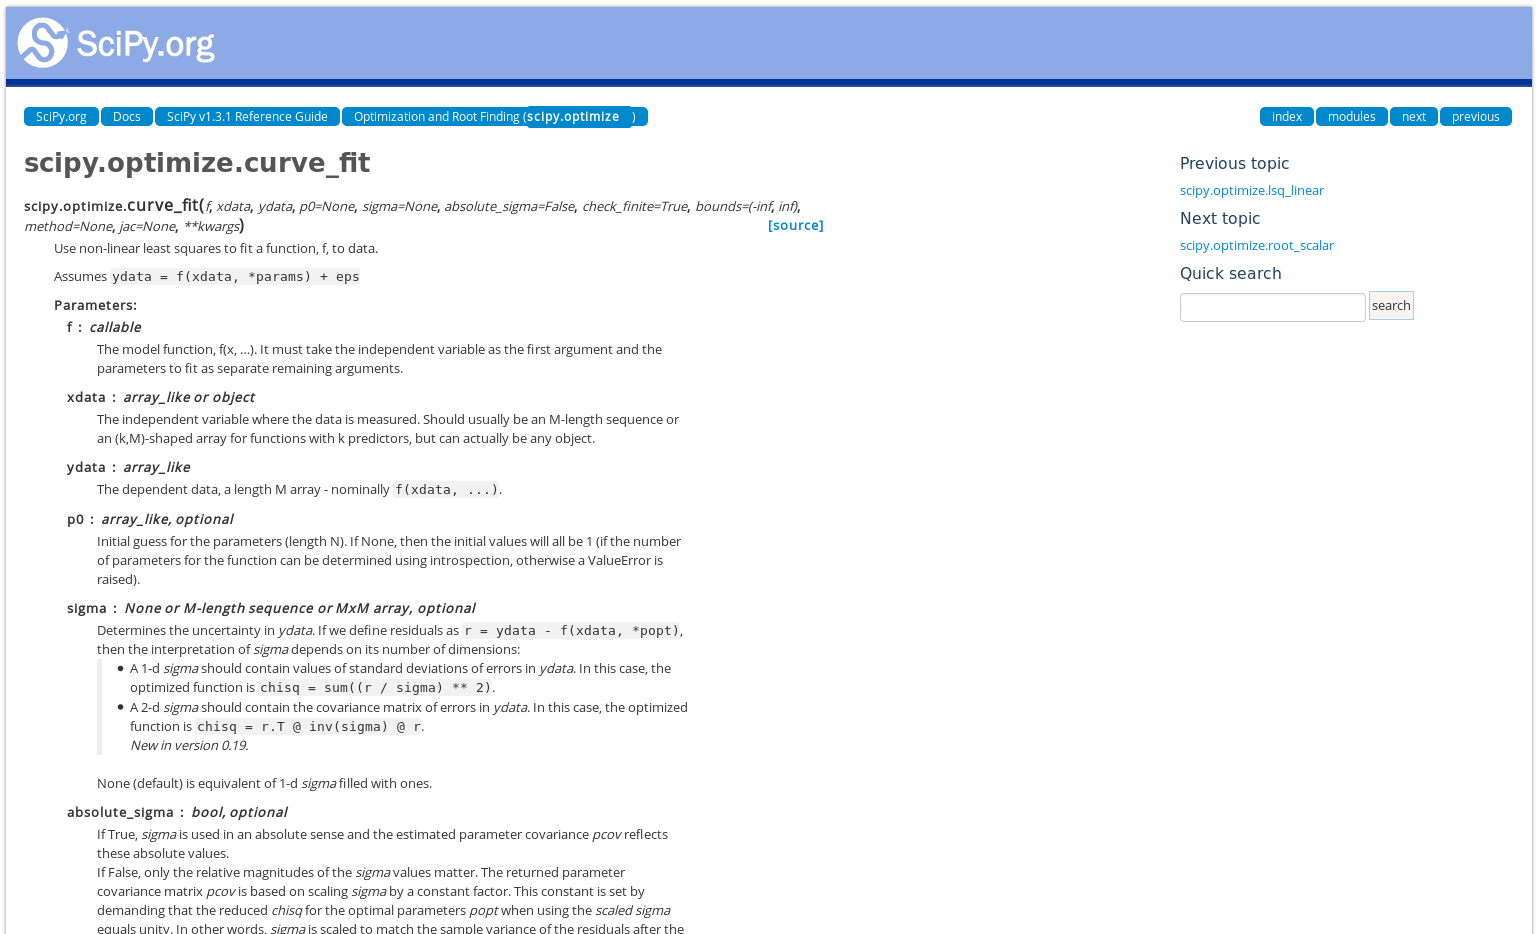
\includegraphics[width=1\textwidth]{lez6/doc_scipy.png}
    \caption{How do the hell they do that?}
    \label{scipy_documentation}
\end{figure}
\FloatBarrier

\begin{figure}[ht]
    \centering
    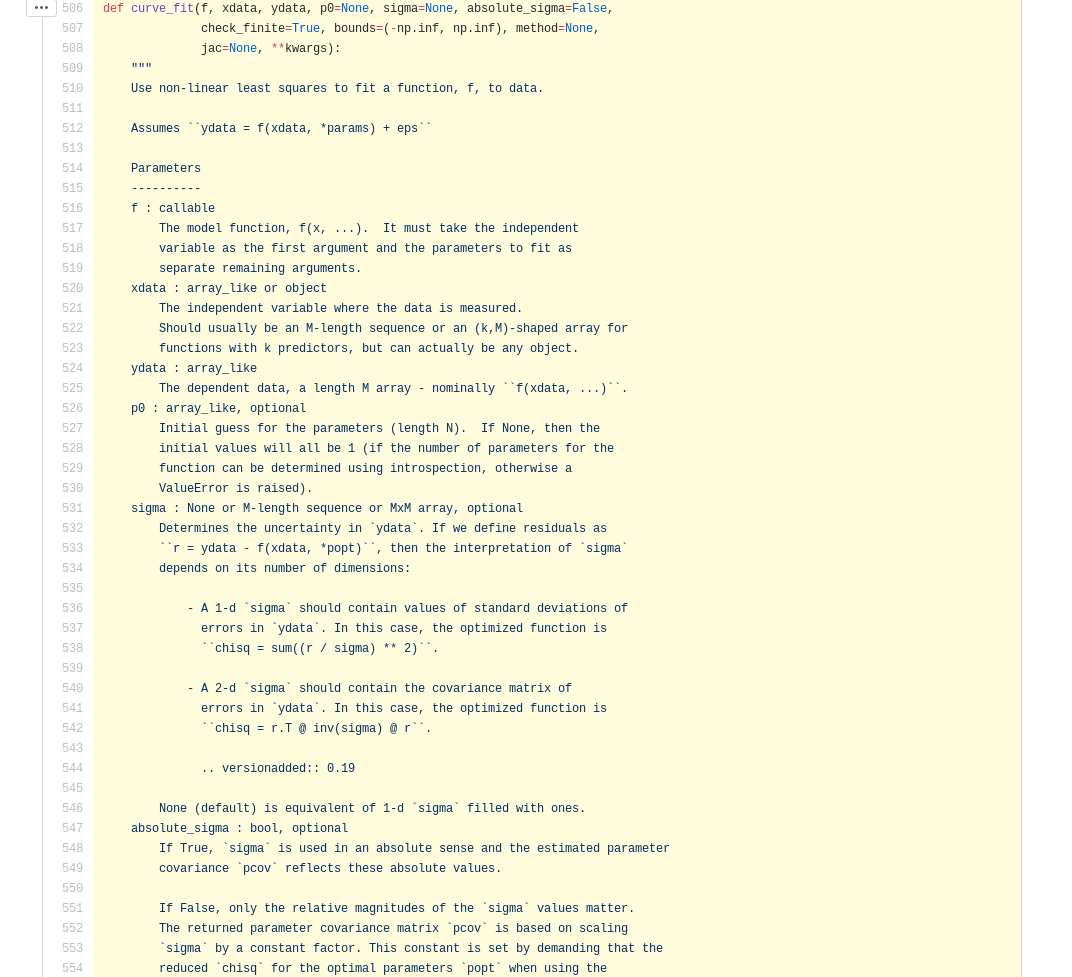
\includegraphics[width=1\textwidth]{lez6/codice_doc.png}
    \caption{the documentation is embedded in the code. . .}
    \label{documentation_code}
\end{figure}
\FloatBarrier

\subsection{Sphinx: the documentation tool for Python}


\subsection{Sphynx basics}

  \begin{itemize}
  \item Process all the relevant information to produce several types of
    output
    \begin{itemize}
    \item Most notably html and LaTeX
    \end{itemize}
  \item Two different sources:
    \begin{enumerate}
    \item The doctrings in the Python modules
    \item Additional markup files (in reStructuredText) containing
      auxiliary information
    \end{enumerate}
  \item Typical workflow:
    \begin{itemize}
    \item Use \texttt{sphinx-quickstart} once when you setup your project
    \item Tweak the generated \texttt{conf.py} file to suit your needs
    \item Go ahead and have fun!
    \end{itemize}
  \item Sphinx is \emph{very} powerful
    \begin{itemize}
    \item e.g., \url{https://docs.python-guide.org/} is written in Sphinx,
      and so is all the Python documentation
    \end{itemize}
  \end{itemize}


\begin{figure}[ht]
    \centering
    
\includegraphics[width=0.9\textwidth]{lez6/sphinx.png}
    \caption{.}
    \label{sphynx}
\end{figure}
\FloatBarrier

\subsection{Ok, I have the documentation compiled, now what do I do with it?}

  \begin{itemize}
  \item Wouldn't it be nice if the documentation was automatically compiled and
    uploaded on the web each time I push on the master?
  \item This is possible and is called readthedocs.com
    \begin{itemize}
    \item And, again, this is a cloud-based service that can interoperate
      easily with github, gitlab or bitbucket
    \end{itemize}
  \end{itemize}


\textbf{NOTA: Per il progetto di fine anno bisogna fare tutto questo, compreso avere la documentazione su un sito come readthedocs}.


\newpage

\section{Torniamo a numpy}
L'ultima volta abbiamo visto il broadcasting.\\

\subsection{Mathematical functions in Numpy}

\inputminted{python}{snippets/numpy_functions.py}

\begin{minted}{bash}
[Output]
[-1. 0. 1.]
[1.10517092e+00 2.71828183e+00 2.20264658e+04]
[ 0.09983342 0.84147098 -0.54402111]
-1.0
Traceback (most recent call last):
    File "snippets/numpy_functions.py", line 12, in <module>
        print(math.log10(a))
TypeError: only size-1 arrays can be converted to Python scalars
\end{minted}

numpy mathematical functions interoperate natively with arrays (and work on plain old numbers, too).

\subsection{Array and Masks}
Masks are a powerful tool in numpy. They can replace conditional expressions in a for loop in vectorization context .

\inputminted{python}{snippets/numpy_masks.py}
\begin{minted}{bash}
[Output]
[ 0. 1. 2. 3. 4. 5. 6. 7. 8. 9. 10.]
[False False False True True True True True True True]
[ True True True True True True True True True False False]
[ 3. 4. 5. 6. 7. 8. 9. 10.]
[0. 1. 2. 3. 4. 5. 6. 7. 8.]
[3. 4. 5. 6. 7. 8.]
\end{minted}

\textbf{Altro esempio:}

\begin{minted}{python}
a = np.random.uniform(size=10)
mask = a > 0.5

mask.sum() #mi restituisce il numero di elementi che soddisano la condizione

#posso passare una maschera tra parentesi quadre per indirizzare gli elementi di un array.
#Mi restituisce un nuovo array contenente solo gli elementi che soddisfano la condizione

a[mask]
\end{minted} 


\textbf{Da fare: guardare come si fa lo slicing di un array}


\subsection{Digression: pseudo-random number generators}

\begin{minted}{python}
import random
x = random.random()
\end{minted}

\begin{itemize}
  \item Every programming language comes with a Pseudo Random Number
    Generator (PRNG)
    \begin{itemize}
    \item Python is no exception:
      \url{https://docs.python.org/3/library/random.html}
    \item Mersenne-Twister, 53-bit precision, period of $2^{19937} - 1$. 
    \end{itemize}
  \item PRNGs are an interesting (and fun) subject by themselves:
    \begin{itemize}
    \item Donald E. Knuth, \emph{The Art of Computer Programming, Volume 2: Seminumerical Algorithms}, 3rd Edition 
    \item M. Matsumoto and T. Nishimura, \emph{Mersenne Twister: A 623-dimensionally equidistributed uniform pseudorandom number generator}, ACM Transactions on Modeling and Computer Simulation Vol. 8, No. 1, January pp.3--30 1998.
    \end{itemize}
  \item A PRNG produces random floats uniformly in $[0.0,~1.0)$.
  \end{itemize}
  
\textbf{Nota} Il modulo random di numpy mi permette di generare numeri random non uno alla volta, ma in array!

\subsection{Vettorizzazione}
Avoid explicit for loops in Python whenever you can!

\textbf{pandas}: utile per leggere e scrivere file excel.

\inputminted{python}{snippets/vectorization.py}
\begin{minted}{bash}
[Output]
Elapsed time: 0.137 s
Elapsed time: 0.015 s
\end{minted}

\subsection{How does vectorizaion work?}


  \begin{itemize}
  \item Python is know to be slooow
    \begin{itemize}
    \item This is the price you pay for being so beautiful and flexible
    \end{itemize}
  \item Does it matter? If depends\ldots
    \begin{itemize}
    \item If you are parsing a text file or fetching a web page probably not
    \item If you are performing a CPU-intensive processing on a TB of data
      probably yes
    \end{itemize}
  \item What's so magic in using numpy?
  \item numpy is written in C as a Python extension
    \begin{itemize}
    \item Routines are highly optimized to cruch numbers
    \item When you perform an array operation in Python you are actually
      executing optimized C code
    \end{itemize}
  \item \alert{Basic message: avoid for loops in pure Python when
    crunching numbers}
  \end{itemize}

\newpage

\section{Secondo Assegnamento}

\subsection{How do I throw PRN with arbitrary pdf?}


\textbf{Hit or miss:}
\begin{center}
  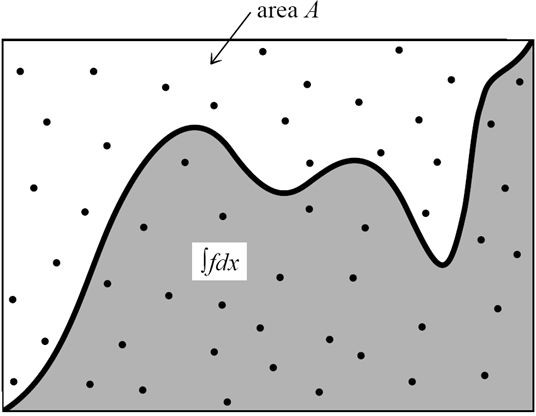
\includegraphics[width=0.5\textwidth]{lez6/hitmiss.jpg}
\end{center}

  \begin{itemize}
  \item Hit or miss, aka acceptance/rejection method:
    \begin{itemize}
    \item Enclose your pdf in a rectangle
    \item Throw a $x$ and a $y$
    \item Accept $x$ if $y \leq f(x)$
    \end{itemize}
  \item \alert{This is horrible---please don't use it!}
  \end{itemize}


\noindent
\textbf{Inverse transform}

  \begin{itemize}
  \item Probability density function (pdf)
    $$
    p(x) \quad (\ge 0)
    $$
  \item Cumulative function (cf)
    $$
    F(x) = \int_{-\infty}^{x} p(x') dx'
    $$
  \item Percent-point function (ppf)
    $$
    x = F^{-1}(q)
    $$
  \item \alert{Awesome fact: if $q$ is uniformly distributed in $[0, 1]$,
    then $x = F^{-1}(q)$ is distributed according to $p(x)$!}
  \end{itemize}

\subsection{An interesting object: splines}
  
\begin{center}
  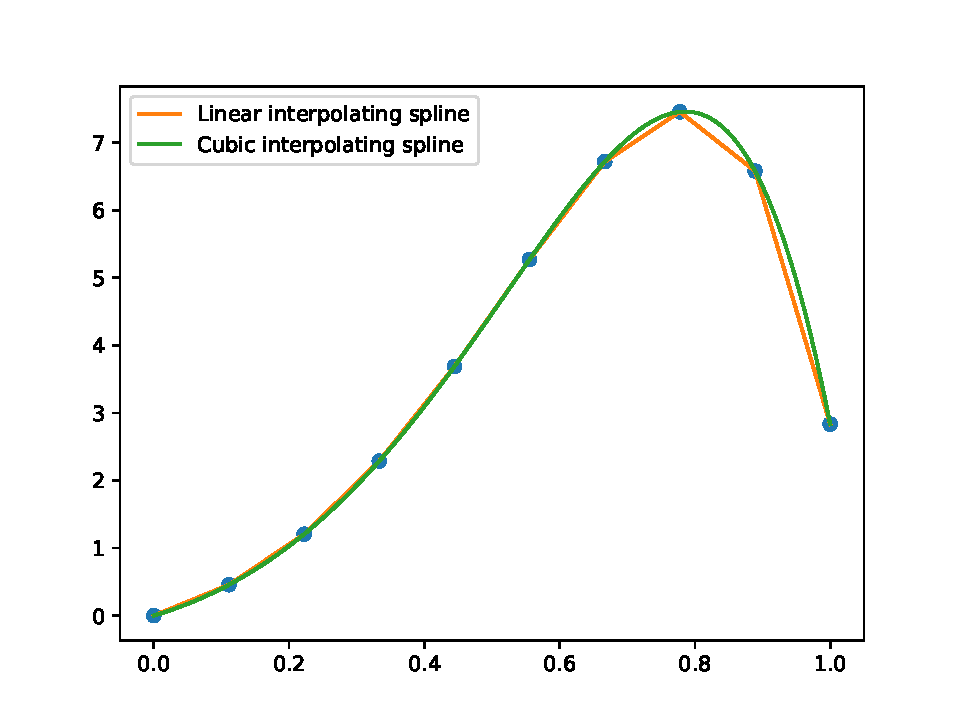
\includegraphics[width=0.7\textwidth]{lez6/spline.pdf}
\end{center}  
  
  \begin{itemize}
  \item Defined piecewsise by polinomials of degree k ($k = 3$ fairly popular)
    \begin{itemize}
    \item Interpolating: passing through a set of pre-defined points
    \item First $k-1$ derivatives continuos at the control points
    \end{itemize}
  \item Superior to polynomial interpolation or curve fitting in many cases
  \end{itemize}

\subsection{Splines: construction and properties}

\inputminted{python}{snippets/spline.py}
\begin{minted}{bash}
[Output]
1.3192110648078448
2.6659857771053925
\end{minted}

  \begin{itemize}
  \item Evaluation is fairly inexpensive
    \begin{itemize}
    \item If the input $x$-array is sorted can do a binary search in
      \alert{O(log(N)) complexity}
    \end{itemize}
  \item Derivatives and integrals are easy
    \begin{itemize}
    \item Can be calculated \emph{exactly} by means of elementary
      arithmetic operations
    \end{itemize}
  \end{itemize}
  
\vfill

\begin{tcolorbox}[width=\textwidth,colback={white},title={References },colbacktitle=gray,coltitle=black]
  \begin{itemize}
  \item \url{https://numpy.org/}
  \item \url{https://www.scipy.org/}
  \item \url{https://docs.scipy.org/doc/numpy/reference/arrays.indexing.html}
  \item \url{https://docs.scipy.org/doc/numpy/user/basics.broadcasting.html}
  \item \url{https://docs.scipy.org/doc/scipy/reference/interpolate.html}
  \end{itemize}
\end{tcolorbox}

\newpage


\section{\textit{Gio 13 ott - Lezione 7}}

\section{Advanced Python Features}

\subsection{Errors and Exceptions}
  \begin{itemize}
    \item \alert{Error handling} is one of the most important problem to solve when designing a program
    \item What should I do when I piece of code fails?
    \item What does fail mean?
    \begin {itemize}
      \item Invalid input e.g. passing a path to a non existent file, or passing a string to a function for dividing numbers
      \item Valid output not found, e.g searching the position of the letter 'd' in the string 'elephant'
      \item Output cannot be find in a reasonable amount of time
      \item Runtime resource failures: network connection down, disk space ended\dots
    \end{itemize}
    \item Two phylosophies (historically):
    \begin{itemize}
      \item Return some \alert{error flag} (in different ways) to tell the user that something went wrong
      \item \alert{Exceptions}
    \end{itemize}
    \item Example: a typical convention for programs is to return 0 from the main if the execution was successful and an
          error code (integer number) otherwise
  \end{itemize}
  


\subsection{Error flags (no)}

\inputminted{python}{snippets/error_flags.py}
\begin{minted}{bash}
[Output]
3
-1
We all live in a
We all live in a Yellow Submarin
\end{minted}

\subsection{Problems of error flags}

    Error codes have their use (and are fine in some cases) but they suffer from a few issues:
    \begin{itemize}
      \item Choosing them is often arbitrary (and sometimes is difficult to make a sensible choice)
      \begin{itemize}
        \item What if all the numbers can represent meaningful output of the function?
      \end{itemize}
      \item Are cumbersome to use
      \begin{itemize}
        \item Which error flag is used by a function? 0? -1? 99999999? $\rightarrow$ you have to go through the documentation for each!
        \item If you have a deep hierarchy of functions you have to perform checks and pass the error up at every level!
      \end{itemize}
      \item What if the caller of a function does not check the error flag?
      \begin{itemize}
        \item The bug can propagate \alert{silently} through its code!
      \end{itemize}
    \end{itemize}
    \medskip
    We want something that:
    \begin{itemize}
      \item Is clearly separated from the returned output
      \item Cannot be silently ignored by the user
      \item Is easy to report to upper level without lots of lines of code
    \end{itemize}  

\subsection{A different way}

\inputminted{python}{snippets/exceptions_vs_err_flags.py}
\begin{minted}{bash}
[Output]
We all live in a
Traceback (most recent call last):
    File "snippets/exceptions_vs_err_flags.py", line 11, in <module>
        print(cut_before(’We all live in a Yellow Submarine’, ’Red’))
    File "snippets/exceptions_vs_err_flags.py", line 5, in cut_before
    pos = input_string.index(substring)
ValueError: substring not found
\end{minted}

La filosofia base di Python è evitare di inventare delle cose.\\
Come faccio ad intercettare questo value error e in quel caso a fargli fare qualcosa di specifico?\\

\subsection{Eccezioni}

  \begin{itemize}
    \item An exception is an object that can be \alert{raised} (in other languages also \textit{thrown}) by
          a piece of code to signal that something went wrong
    \item When an exception is raised the normal flow of the code is interrupted
    \item The program automatically propagate the exception back in the function hierarchy
          until it found a place where the exception is  \alert{catched} and handled
    \item If the exception is never catched, not even in the main, the program crash \alert{with a specific error message}
    \item Cathcing the exception is done with a \emph{try - except} block
  \end{itemize}
  
Se non intercettiamo l'eccezione, il flusso del codice viene interrotto.
Possiamo dire "se ho questa eccezione allora faccio questo...".

\subsection{Try block}


\inputminted{python}{snippets/exceptions_brief.py}
\begin{minted}{bash}
[Output]
This line is not executed if an exception is raised in the try block
This line is executed only if a ValueError is raised in the try block
\end{minted}

Per ogni try possiamo anche mettere più di un except.\\
Dobbiamo cercare di intercettare le eccezioni nel modo più specifico possibile!

\subsection{\texttt{else}, \texttt{finally}}

  \begin{itemize}
    \item There are two more optional statements in a try-block:
    \medskip
    \begin{itemize}
      \item \emph{else}: executed only if no exception is raised in the try block
      \medskip
      \item \emph{finally}: executed no matter what
      \medskip
    \end{itemize}
    \item \emph{finally} is executed even if there is a return statement in the try
          block
    \item can be used to release important resources (e.g. closing a
          file, or a connection)
  \end{itemize}

\subsection{Using \texttt{else} and \texttt{finally}}

\inputminted{python}{snippets/exceptions.py}
\begin{minted}{bash}
[Output]
This line
This line
This line
This line
This line
A. Manfreda (INFN)
is
is
is
is
is
not executed if an exception is raised in the try block
executed only if no exception is raised in the try block
always executed
executed only if a ValueError is raised in the try block
always executed
\end{minted}


L'eccezione è un oggetto. E dentro di essa possiamo encapsulare tutte le informazioni necessarie per capire cosa è andato storto!



\subsection{The beauty of exceptions}
  \begin{itemize}
    \item If that was all, exceptions would only be moderately useful
    \item The real bargain is that you can send back information together with the exception
    \item In fact you \textit{are sending a full object}: the excetpion iteslf. Surprised?
    \item Inside the exception you can report all kind of data useful to reconstruct the exact error,
          which can be used by the caller for debug or to produce meaningful error messages
    \item You can also select which exceptions you catch, leaving the others propagate up
    \item Python provides a rich hierarchy of exception classes, which you can further customize
          (if you want) by deriving your own subclasses
  \end{itemize}

\subsection{The family tree of Python exceptions}

\begin{figure}[ht]
    \centering
    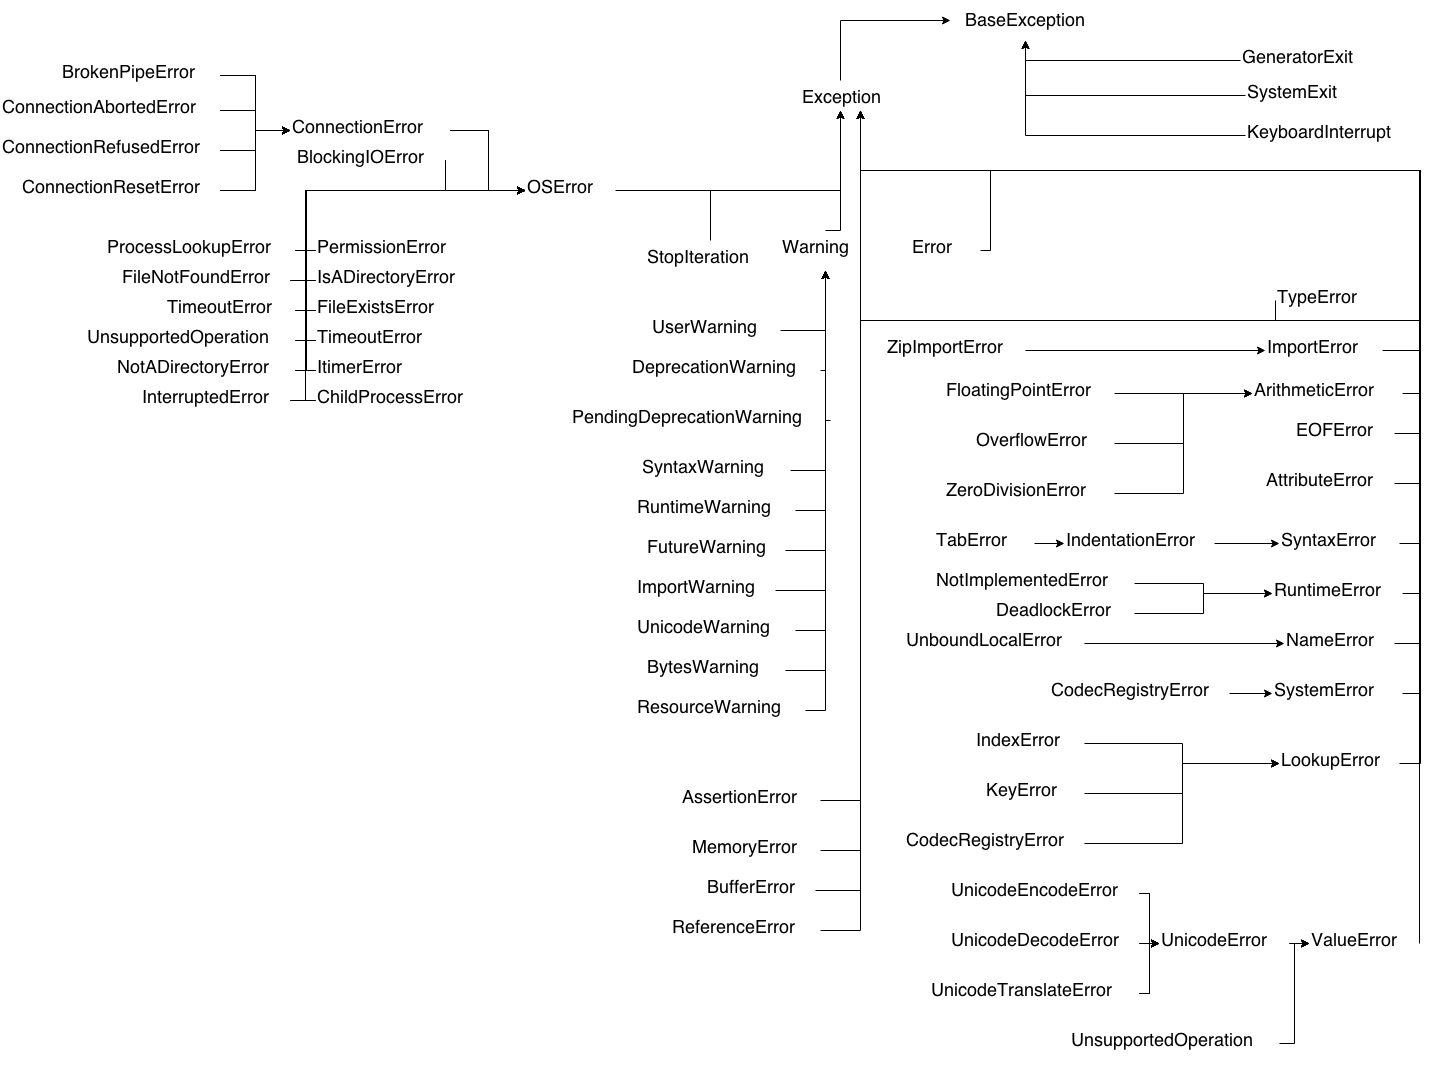
\includegraphics[width=1\textwidth]{lez7/error_tree.png}
    \caption{family tree}
    \label{error_tree}
\end{figure}
\FloatBarrier


\subsection{Catching specific exceptions}

\inputminted{python}{snippets/try_block.py}
\begin{minted}{bash}
[Output]
[Errno 2] No such file or directory: ’i_do_not_exist.txt’
\end{minted}

\texttt{Exception} sta per qualsiasi altro tipo di errore.


\subsection{Exception caveats}
  \begin{itemize}
    \item Warning: catching \emph{Exception}, will also catch \emph{SyntaxError}
          and \emph{NameError}
    \medskip
    \item This mean that the code will 'run' even if there is a typo in it!
    \medskip
    \item Bottom line: \alert{you should never catch generically for \emph{Exception}},
          always be more specific
    \medskip
    \item Even worse, you should never catch for \emph{BaseException} as
          that would even prevent the user for from aborting the execution with a
          \emph{KeyboardInterrupt} (e.g. Ctrl-C)
    \medskip
    \item Unless that is what you need, of course
  \end{itemize}
  
  
  \subsection{There is no check - only try}
  \begin{itemize}
    \item In Python exceptions are the default methods for handling failures
    \smallskip
    \item Many functions raise an exception when something goes wrong
    \smallskip
    \item The common approach is: do not chech the input beforehand. Use it and
          be ready to catch exceptions if any.
    \smallskip
    \item \textit{Easier to ask for forgiveness than permission.} 
  \end{itemize}
  
  
\subsection{Catching specific exceptions}

\inputminted{python}{snippets/dont_ask_permission.py}
\begin{minted}{bash}
[Output]
Oops - file ’i_do_not_exists.txt’ does not exist
Oops - cannot read the file!
[Errno 2] No such file or directory: ’i_do_not_exists.txt’
\end{minted}


%%%%% slide saltate


\subsection{Raising exceptions}
  \begin{itemize}
    \item Up to now we have been dealing with exceptions generated by Python
          functions
    \medskip
    \item What about raising exceptions ourselves?
  \end{itemize}
  
\inputminted{python}{snippets/raising.py}
\begin{minted}{bash}
[Output]
this is a useful debug message
\end{minted}

Valutare bene prima di mettere \texttt{sys.exit('guarda che ho bisogno di quel file')}. Se invece sollevo un'eccezione, offro la scelta a chi esegue il codice.\\

\subsection{Custom exceptions}
  \begin{itemize}
    \item Beside the built-in exceptions provided by Python, you can add your
          own custom exceptions by inheriting from the \emph{Exception} class
    \medskip
    \item This serves two purposes:
    \begin{itemize}
      \item Make the exception handling code more specific, and hence more
            readible
      \item Allows you to pass additional data with your exception - in the
            form of attributes of the class - which can be used for debug
            or any other purpose
    \end{itemize}
  \end{itemize}

\inputminted{python}{snippets/custom_exceptions.py}
\begin{minted}{bash}
[Output]
Traceback (most recent call last):
File "snippets/custom_exceptions.py", line 4, in <module>
raise SimpleCustomError(’simple error’)
__main__.SimpleCustomError: simple error
\end{minted}

\textbf{altro esempio:}

\inputminted{python}{snippets/custom_exceptions_2.py}
\begin{minted}{bash}
[Output]
ValueTooLargeError: 100 is too large
\end{minted}


\subsection{Where to catch exceptions?}
  \begin{itemize}
    \item Differently from error flags, which need to be checked as early as
          possible, you are not in a rush with exceptions
    \item Remeber: your goal is to provide the user a meaningful error message and
          useful debug information.
    \item You should catch an exception only when you have enough context to
          do that - which sometimes means waiting a few levels in the hierarchy!
  \end{itemize}

I blocchi try-except devono essere il più piccolo possibile, e il più specifico possibile!

%%%%%%

\subsection{When to catch}

\inputminted{python}{snippets/when_to_catch.py}
\begin{minted}{bash}
[Output]
0.1 15.2
0.2 12.4
Traceback (most recent call last):
File "snippets/when_to_catch.py", line 12, in <module>
time, tension = parse_line(line)
File "snippets/when_to_catch.py", line 6, in parse_line
tension = float(values[1])
ValueError: could not convert string to float: ’pippo’
\end{minted}

\subsection{Catch too early}

\inputminted{python}{snippets/when_to_catch_1.py}
\begin{minted}{bash}
[Output]
0.1 15.2
0.2 12.4
could not convert string to float: ’pippo’
Traceback (most recent call last):
File "snippets/when_to_catch_1.py", line 15, in <module>
time, tension = parse_line(line)
TypeError: ’NoneType’ object is not iterable
\end{minted}

\subsection{Catch when needed}

\inputminted{python}{snippets/when_to_catch_2.py}
\begin{minted}{bash}
[Output]
0.1 15.2
0.2 12.4
Line 3 error: could not convert string to float: ’pippo’
0.4 13.2
\end{minted}

\newpage
\section{\textit{Lun 17 ott - Lezione 8}}

\section{Iterators}

Quando una classe implementa il metodo \texttt{\_\_iter\_\_} allora diventa \textit{iterabile}.

  \subsection{Iterators and iterables}
Un iteratore è un oggetto definito dal fatto di sapere qual è il prossimo elemento, grazie al metodo magico \texttt{\_\_next\_\_}.  

  \begin{itemize}
    \item An \emph{iterable} in Python is something that has a \emph{\_\_iter\_\_}
          method, which returns an \alert{iterator}
    \item An \emph{iterator} is an object that implement a \emph{\_\_next\_\_} method
          which is used to retrieve elements one at the time
    \item When there are no more elements to return, the iterator signals that with a specific
          exception: \emph{StopIteration()}
    \item An iterator also implement an \emph{\_\_iter\_\_} method that return\dots itself.
          So an iterator is also technically an iterable%
          \footnote{Only 'technically' because an iterator has no data of its
          own, so you always need a 'real' iterable to actually iterate}%
          ! (But the opposite is not true)
  \end{itemize}

Perché passare dall'iteratore? Perché non implementare il metodo \texttt{\_\_next\_\_} direttamente sul nostro oggetto? Il fatto è che posso avere più iteratori attivi su uno stesso contenitore dati. Per questo non posso implementare il metodo \texttt{\_\_next\_\_} direttamente nella classe di dati, ma devo passare per l'iteratore.

\subsection{A 'for' loop unpacked}

\inputminted{python}{snippets/show_iterator.py}
Salvo il mio iteratore in una variabile e inizio un ciclo (potenzialmente infinito). Quando l'iterazione solleva l'eccezione \texttt{StopIteration} interrompo il ciclo.
\begin{minted}{bash}
[Output]
1.0
2.0
3.0
1.0
2.0
3.0
\end{minted}

\subsection{A simple iterator}


\inputminted{python}{snippets/simple_iterator.py}
Nel costruttore gli passo il contenitore di dati su cui voglio iterate. Mi salvo una referenza a questo contenitore dati. E faccio partire l'indice da zero.
Nota: questo funziona per le liste, tuple e array, ma non per i dizionari, che non restituiscono \texttt{indexError}, ma \texttt{KeyError}!


\inputminted{python}{snippets/test_simple_iterator.py}

\begin{minted}{bash}
[Output]
1.0
2.0
3.0
stella
\end{minted}

\subsection{A crazy iterator}
\inputminted{python}{snippets/crazy_iterator.py}

\inputminted{python}{snippets/test_crazy_iterator.py}

\begin{minted}{bash}
[Output]
B
E
A
C
A
D
D
D
\end{minted}

\subsection{Python tools for iterables}

  \begin{itemize}
    \item Python provides a number of functions that consume an iterable and return a single value:
    \begin{itemize}
      \item \texttt{sum}: Sum all the elements
      \item \texttt{all}: Return true if a given condition is true for all the elements
      \item \texttt{any}: Return true if a given condition is true for at lest one element
      \item \texttt{max}: Return the max
      \item \texttt{min}: Return the minimum
      \item \texttt{functools.reduce}: Apply a function recursively to pairs of elements
    \end{itemize}
  \end{itemize}

\section{Generatori}

Gli iteratori operano su dati \textbf{esistenti}. Tuttavia, a volte vorremmo iterare su qualcosa che non esiste già da prima. Ad esempio, se vogliamo generare in maniera iterativa tutti i numeri della serie di Fibonacci; ad ogni iterazione vogliamo generare il prossimo.\\
Questa cosa non si può fare con gli iteratori, ma si fa con i \textbf{generatori}:\\\

  \begin{itemize}
    \item We have seen that iterators are useful to iterate over container
    \item However that assumes a containers exists $\rightarrow$ memory usage
    \item \alert{Generators} allow you to loop over sequences of items even when
          they don't exist before - the items are just created \alert{lazily} the
          moment they are required (\textbf{lazy:} una cosa che viene fatta all'ultimo momento possibile.)
    \item For example you can write a generator to loops over the Fibonacci
          succession. You can't create the sequence earlier, since it is not
          finite!
    \item Generators are created through either \alert{generator expressions} or
          \alert{generator functions}
    \item In real life most of the time you will simply use pre-made functions
          that return a generator, like \emph{range()} (in Python 3)
    \item Generator can be used to iterate in for loops, just like iterators
  \end{itemize}


\subsection{Generators first look}

Sui generatori possiamo iterare esattamente come sugli iteratori: la sintassi è la stessa.\\

\inputminted{python}{snippets/generators.py}

\begin{minted}{bash}
[Output]
0
1
2
3
144
1
25
\end{minted}


\subsection{Generator functions}

  \begin{itemize}
    \item A \alert{generator function} is a function that contains the keyword \alert{yield} at
          least once in his body
    \item When you call a generator function the code is not executed - instead
          a generator object is created and returned (even if you don't have a return statement)
    \item Each call to \emph{next()} on the returned generator will make the function code 
          run until it finds a \emph{yield} statement
    \item Then the execution is paused and the value of the expression on the right 
          of \emph{yield} is returned (yielded) to the caller
    \item A further call of next will resume the execution from where it was suspended
          until the next \emph{yield} and so on
    \item Eventually, when the function body ends, \emph{StopIteration} is raised
    \item Usually generators functions contain a loop - but it's not mandatory!
  \end{itemize}

Quando noi chiamiamo una funzione generatrice, non viene eseguito il corpo della funzione, bensì viene restituito un generatore.

\inputminted{python}{snippets/generator_functions.py}

\begin{minted}{bash}
[Output]
First call
1
Second call
2
I am about to rise a StopIteration exception...
Traceback (most recent call last):
    File "snippets/generator_functions.py", line 11, in <module>
        next(gen) # The third next() will throw StopIteration
StopIteration
\end{minted}


\subsection{Infinite sequence generators}

Tipicamente all'interno del generatore c'è un loop.

\inputminted{python}{snippets/fibonacci.py}

\begin{minted}{bash}
[Output]
[0, 1, 1, 2, 3, 5, 8]
[0, 1, 1, 2, 3, 5, 8]
\end{minted}

islice prende un certo numero di elementi da un iteratore.\\

Un generatore serve in tutti quei casi in cui voglio generare i vari elementi in maniera lazy.\\

  \subsection{Python generator functions}
  
  \begin{itemize}
    \item Python provides a number of built-in functions that return a generator from an iterable, such as:
    \begin{itemize}
      \item \texttt{enumerate}: Automatic counting of iterations
      \item \texttt{map}: Apply a function to the elements
      \item \texttt{filter}: Return only the elements passing a given condition
      \item \texttt{zip}: Return pairs of elements (requires two sequences)
      \item \texttt{reversed}: Loop in the reversed order
    \end{itemize}

    \item Countless others can be found in the \alert{\texttt{itertools}} library
    \begin{itemize}
      \item \texttt{islice}: Slice the loop with start, stop and step
      \item \texttt{takewhile}: Stop looping when a condition becomes false
      \item \texttt{accumulate}: Get the results of applying the function iteratively to pair of elements
      \item \texttt{chain}: Loop through many sequences one after another
      \item \texttt{cycle}: Loop over the sequence repeatedly, indefinitely
      \item \texttt{permutations}: Get all the permutations of a given length
      \item \texttt{product}: Compute the cartesian product of iterables
      \item \texttt{groupby}: Group by value of some key (function)     
      \item And so on\dots
    \end{itemize}
    
    \medskip
    
    \item Take a look at the documentation of each function to see how to 
          properly call it!
  \end{itemize}  

\subsection{Itertools showcase}

\inputminted{python}{snippets/itertools_showcase.py}

\begin{minted}{bash}
[Output]
[1, 3, 6, 10]
[1, 2, 6, 24]
[(1, 2, 3), (1, 2, 4), (1, 3, 4), (2, 3, 4)]
[(5, 6), (6, 5)]
[(1, 5), (1, 6), (2, 5), (2, 6), (3, 5), (3, 6), (4, 5), (4, 6)]
False [1, 3, 5]
True [2, 4, 6]
\end{minted}

\section{Lambda functions}

Sono un modo per creare una funzione anonima (senza un nome).

  \begin{itemize}
    \item \alert{Anonymous functions}, or \alert{lambda functions} are a construct typical of \alert{functional programming}
    \item \url{https://en.wikipedia.org/wiki/Lambda_calculus}
    \item \url{https://en.wikipedia.org/wiki/Functional_programming}
    \item In Python a lambda function is essentially a special sintax for creating a function
          on the fly, without giving it a name
    \item They are limited to \alert{a single expression}, which is returned to the user
    \item Many of the typical uses for lambdas are already covered in python by generator expressions and comprehension,
          so this is more like a niche feature of the language
  \end{itemize}
  

\inputminted{python}{snippets/lambda.py}
Il corpo di una funzione deve essere solo una riga.\\
\texttt{lambda argomenti: output}
\begin{minted}{bash}
[Output]
-5
[0, 1, 4, 9, 16, 25, 36, 49, 64, 81]
[0, 1, 4, 9, 16, 25, 36, 49, 64, 81]
\end{minted}

\subsection{Recap example: file iterator}

\inputminted{python}{snippets/file_iterator.py}

\begin{minted}{bash}
[Output]
0 0.1 15.2
1 0.2 12.4
Line 1 error: could not convert string to float: ’pippo’
\end{minted}

\subsection{File iterator redone}


\inputminted{python}{snippets/file_iterator_2.py}

\begin{minted}{bash}
[Output]
0.1 15.2
0.2 12.4
Line 3 error: could not convert string to float: ’pippo’
0.4 13.2
\end{minted}


\subsection{File iterator, final version}

\inputminted{python}{snippets/file_iterator_3.py}

\begin{minted}{bash}
[Output]
0.1 15.2
0.2 12.4
Line 3 error: could not convert string to float: ’pippo’
0.4 13.2
\end{minted}

\section{Decorators}
\textit{non ha avuto tempo di farli tutti, vediamo solo:}
  \subsection{The @classmethod decorator}
costruttore alternativo
  \begin{itemize}
    \item We have already seen a built-in Python decorator: \emph{@property}
    \item We used that to get proper encapsulation
    \item There is another built-in decorator one which is very useful for classes: \alert{\emph{@classmethod}}
    \item A classmethod is like a class attribute: you don't need an instance to
          use it
    \item A class method can access class attributes but not instance attributes
    \item The main use for class methods is to provide \alert{alternate constructors}
  \end{itemize}


\inputminted{python}{snippets/classmethod.py}

\begin{minted}{bash}
[Output]
<class ’__main__.LabData’>
[15.2 12.4 11.7 13.2]
\end{minted}


